 % main file
\documentclass[12pt, twoside, a4paper, openright]{book}
\newcommand{\egilea}{Mikel Balduciel Diaz}
\newcommand{\izenburua}{Baldugenda}
\newcommand{\data}{2015ko maiatzaren 27}
\newcommand{\myparagraph}[1]{\paragraph{#1}\mbox{}\\}
\usepackage{subfig}
\usepackage{float}
\usepackage{wrapfig}
\usepackage{booktabs}
\usepackage{graphicx}
\usepackage{tikz}
\usetikzlibrary{arrows.meta}
\usetikzlibrary{calc}
\usetikzlibrary{babel}

% \newcommand{\euskaraz}{eu} % Comentar para castellano

% Nota Importante: En el caso de castellano, la codificación de los archivos
% deberá ser utf-8

% Codificación del archivo / fitxategiaren kudeaketa
\usepackage{ucs}
\usepackage[utf8x]{inputenc}
\usepackage[T1]{fontenc}


% ################################################################
% #######     SIZE OF THE PAGES                     ##############
% ################################################################
\usepackage[left=3.5cm, right=2.5cm, top=4.0cm, bottom=3.0cm]{geometry}
% \usepackage[left=1.5cm, right=2.5cm, top=2.0cm, bottom=2.0cm]{geometry}


% ################################################################
% #######     HEADERS                               ##############
% ################################################################
\usepackage{fancyhdr}           % Para cambiar las cabeceras de las pginas

\pagestyle{fancy}
\renewcommand{\chaptermark}[1]{ \markboth{#1}{} }
\renewcommand{\sectionmark}[1]{ \markright{#1}{} }

\fancyhf{}
\fancyhead[LE,RO]{\thepage}
\fancyhead[RE]{\textit{ \nouppercase{\leftmark}} }
\fancyhead[LO]{\textit{ \nouppercase{\rightmark}} }

\fancypagestyle{plain}{ %
  \fancyhf{} % remove everything
  \renewcommand{\headrulewidth}{0pt} % remove lines as well
  \renewcommand{\footrulewidth}{0pt}
}


	% Redefine plain page style
	\fancypagestyle{plain}{
		\fancyhf{}
		\renewcommand{\headrulewidth}{0pt}
		\fancyfoot[LE,RO]{\thepage}
	}

	% Define pagestyle
	\pagestyle{fancy}
	\fancyhf{}
	% \renewcommand{\chaptermark}[1]{\markboth{ \emph{#1}}{}}
	\fancyhead[LO]{}
	\fancyhead[RE]{\leftmark}
	\fancyfoot[LE,RO]{\thepage}

	% Code for creating empty pages
	% No headers on empty pages before new chapter
	% \makeatletter
	% \def\cleardoublepage{\clearpage\if@twoside \ifodd\c@page\else
		% \hbox{}
		% \thispagestyle{plain}
		% \newpage
		% \if@twocolumn\hbox{}\newpage\fi\fi\fi}
	% \makeatother \clearpage{\pagestyle{plain}\cleardoublepage}

	% Otra opción: considerar si funciona
	% this next section (till \makeatother) makes sure that blank pages
	%% are actually completely blank, cause they're not usually
	\makeatletter
	\def\cleardoublepage{\clearpage\if@twoside \ifodd\c@page\else
		\hbox{}
		\vspace*{\fill}
		\thispagestyle{empty}
		\newpage
		\if@twocolumn\hbox{}\newpage\fi\fi\fi}
	\makeatother


	% \pagestyle{fancy}				% use fancyhdr style
	% \setlength{\headheight}{13pt}

	% Limpiar estilo actual
	% \fancyhead{}
	% \fancyfoot{}
	% % or \fancyhf{}

	% \renewcommand{\headrulewidth}{0.4pt}    % Cabecera: subraya la cabecera (fijar en "0pt" si no se desea).
	% \renewcommand{\footrulewidth}{0pt}      % Pié: subraya el pie de página (fijar en "0pt" si no se desea).

	% There are seven letters you need to know before you can define your own header/footer:
	% E: Even page
	% O: Odd page
	% L: Left field
	% C: Center field
	% R: Right field
	% H: Header
	% F: Footer

% 	\fancyhead[CO,CE]{---Draft---}
% 	\fancyfoot[CO,CE]{Confidential}

% 	\fancyfoot[RO, LE] {\thepage}
% 	% or \fancyhf[FRO,FLE]...
% 
% 	\fancyhead[RE]{\nouppercase{\leftmark}}	% Cabecera: incluye información del nivel superior (Capítulo) % a la derecha (R) de las páginas pares (E), evitando escribir % todo en mayúsculas (que sería la opción por defecto).
% 	% or \fancyhf[HRE]...
% 
% 	\fancyhead[LO]{\nouppercase{\rightmark}}% Cabecera: incluyer información del nivel inferior (Sección) % a la izquierda (L) de las páginas impares (O), evitando escribir % todo en mayúsculas (que sería la opción por defecto).

	% \renewcommand{\chaptermark}[1]{%
		% \markboth{\small\slshape\chaptername{} \thechapter: #1}{}
		% }
	% \renewcommand{\sectionmark}[1]{%
		% \markright{\small\slshape\thesection : #1}
		% }

\renewcommand{\chaptermark}[1]{\markboth{#1}{}}
\renewcommand{\sectionmark}[1]{\markright{\thesection\ #1}}


%% which sections are numbered
\setcounter{secnumdepth}{2}

 
% ################################################################
% #######     Bibliografia                          ##############
% ################################################################
%\usepackage{natbib}
 %\newcommand{\citenp}[2][ ]{\citeauthor{#2}#1 (\citeyear{#2})}
 %\bibpunct{}{}{;}{a}{,}{,~}
 %\newcommand{\myetal}{\emph{et~al.}}
%\bibliographystyle{plainnat4}
%\bibliographystyle{apalike}
\bibliographystyle{plain}


% To insert development comments (todos, corrections...)
\usepackage[textsize=scriptsize,textwidth=2cm]{todonotes}
% How to use: 
% - \todo{comentario/iruzkina} (insert into tex)
% - \todo[inline]{}

% ################################################################
% #######     FONT TYPES                            ##############
% ################################################################
% Charter
%\usepackage[bitstream-charter]{mathdesign}
% 	\renewcommand{\rmdefault}{mdbch} % charter
\DeclareSymbolFont{usualmathcal}{OMS}{cmsy}{m}{n}
\DeclareSymbolFontAlphabet{\mathcal}{usualmathcal}
%\{charter}
% \renewcommand{\rmdefault}{bch}
% \renewcommand{\bfdefault}{b}

% times erabili beharrean
\usepackage{mathptmx}
\usepackage[scaled=.90]{helvet}

% \renewcommand{\rmdefault}{ppl}
% \usepackage{mathpazo} % palatino
% \linespread{1.05}        % Palatino needs more leading
% \usepackage[bitstream-charter]{mathdesign}
% \usepackage{libertine}

%\usepackage[scaled]{berasans}

%\usepackage[scaled]{beramono}
% \renewcommand{\sfdefault}{fxbf}
	% libertine
% 		\renewcommand{\rmdefault}{fxlj} % Linux libertine 


% Sans serif


% ################################################################
% #######     GRAPHICS                              ##############
% ################################################################
\usepackage{graphicx}
\DeclareGraphicsExtensions{.png,.gif,.jpg,.pdf}
% \graphicspath{./irudiak/}
% \newcommand{\irudia}[3]{%
	% \begin{figure}[htb!]
	% \centering%
	% \includegraphics[width=#2]{#1}
	% \caption{#3}
	% \label{fig:#1}
	% \end{figure}
% }

\usepackage[figuresright]{rotating}

\newcommand{\fitx}[1]{\texttt{#1}}

%%%%%%%%%%%%%%%%%%%%%%%%%%%%%%%%%%%%%%%%%%%%%%%%%%%%%%%%%%%%%%%%
%%%%%%%%%%%  PARRAFOEN ESTILOA    %%%%%%%%%%%%%%%%%%%%%%%%%%%%
\frenchspacing
\widowpenalty=1000

% \titlespacing{\section}{1pc}{0ex plus .1ex minus .2ex}{1pc}
% \titlespacing{\section}{0pt}{*1}{*1}
\setlength{\parindent}{0cm} % anula indentacion de parrafos
\setlength{\parskip}{1.5ex plus 0.5ex minus 0.5ex}   % establece separacion entre parrafos a 8 puntos

\setlength\headheight{15pt}

\usepackage{setspace} % Lerroen arteko espazioa
%\singlespacing
\onehalfspacing
%\doublespacing
%\setstretch{1.1}

% hobeto ``justifika''tzeko
%\usepackage[protrusion=true,expansion=true]{microtype}


%%%%%%%%%%%%%%%%%%%%%%%%%%%%%%%%%%%%%%%%%%%%%%%%%%%%%%%%%%%%%%%%
%%%%%%%%%%% IZENBURUEN ESTILOA   %%%%%%%%%%%%%%%%%%%%%%%%%%%%
\usepackage[sf,outermarks]{titlesec}
% \usepackage[compact]{titlesec}

\titleformat{\chapter}[display]
  {\bfseries\Large}
  {\Large\MakeUppercase{\chaptertitlename} \filleft\Huge\thechapter.}
  {4ex}
  {\titlerule
	\vspace{2ex}%
	\filright}
  [\vspace{2ex}%
   \titlerule]

% ATalen formatua
\renewcommand{\thepart}{\arabic{part}}
\titleformat{\part}[display]
  {\bfseries \Large}
  {\filcenter \Huge\thepart. \Huge\MakeUppercase{\partname}}
  {4ex}
  {%marra
    \vspace{2ex}%
    \filcenter \huge  \filright} %filcenter
  [\vspace{2ex}%
   ]





%usepackage{calc} % para hacer calculos al establecer las medias ej: \textwidth -2px
% \usepackage{sectsty}
% \newcommand{\cabecerasformatosection}[1]{%
	% {\makebox[0.98\linewidth][l]{#1}}
% }
% \newcommand{\cabecerasformatosubsection}[1]{%
	% {\makebox[0.98\linewidth][l]{\textsl{#1}}}
% }
% \newcommand{\cabecerasformatosubsubsection}[1]{%
	% {\framebox[1.1\width][l]{#1}}
% }
% \sectionfont{\cabecerasformatosection}
% \subsectionfont{\cabecerasformatosubsection}
% \subsubsectionfont{\cabecerasformatosubsubsection}
% \sectionfont{\sffamily}
% \subsectionfont{\sffamily\textsl}
% \subsubsectionfont{\sffamily}

\usepackage[hyperindex,pagebackref=true,bookmarks,colorlinks=true,citecolor=blue,urlcolor=blue,linkcolor=blue,pdftex,unicode]{hyperref}
\usepackage{appendix}
\usepackage[acronym,toc,savenumberlist,counter=page]{glossaries} 
%\usepackage{glossaries} 
% Erabilera 
% http://en.wikibooks.org/wiki/LaTeX/Glossary
% latexmk erabiliz gero, ikusi http://tex.stackexchange.com/questions/1226/how-to-make-latexmk-use-makeglossaries

% Glosario-en eskuliburu zabaldua
% http://osl.ugr.es/CTAN/macros/latex/contrib/glossaries/glossaries-user.html#x1-140002.2



\usepackage{color}  
\usepackage{xcolor}
\usepackage{colortbl}

\definecolor{light-gray}{cmyk}{0,0,0,.3} 
\definecolor{orange}{rgb}{1,0.7,0}
\definecolor{light-brown}{RGB}{184,134,11}

\definecolor{gray90}{gray}{.90}
\definecolor{gray75}{gray}{.75}
\definecolor{gray95}{gray}{.95}

\definecolor{lightgray}{gray}{.8}
\definecolor{lightlightgray}{gray}{.95}

\definecolor{atzekokolorea}{gray}{.97}
\definecolor{atzekokoloreasol}{gray}{.7}
\definecolor{atzekokoloreafitx}{gray}{.97}
\definecolor{atzekokoloreafitx_markoa}{gray}{.65}

\usepackage{textcomp} % XML kodea formateatzeko

\usepackage{listings}

\lstset{
    tabsize=4,
    basicstyle=\scriptsize,
    upquote=true,
    aboveskip={1.5\baselineskip},
    columns=fixed,
    showstringspaces=false,
    extendedchars=true,
    breaklines=true,
    showtabs=false,
    showspaces=false,
    showstringspaces=false,
    identifierstyle=\ttfamily,
    commentstyle=\color[rgb]{0.133,0.545,0.133},
    stringstyle=\color[rgb]{0.627,0.126,0.941}\ttfamily,
    morekeywords={SCORE},keywordstyle=\color{red},
    emph={SCORE,CODE,ID,LEMA,POS},emphstyle=\color{light-brown},
    moreemph={[2]top,num,ENtitle,TERM,WF,SYNSET,ENdesc,ENnarr,EStitle,ESdesc,ESnarr,EXP,DOC,DOCNO,DOCID,HEADLINE,TEXT},emphstyle={[2]\color{blue}}
}



\lstset{ frame=Ltb,
     framerule=0pt,
     aboveskip=0.5cm,
     framextopmargin=3pt,
     framexbottommargin=3pt,
     framexleftmargin=0.4cm,
     framesep=0pt,
     rulesep=.4pt,
     backgroundcolor=\color{gray90},
     rulesepcolor=\color{black},
     %
     stringstyle=\ttfamily,
     showstringspaces = false,
     basicstyle=\small\ttfamily,
     commentstyle=\color{gray45},
     keywordstyle=\bfseries,
     %
     numbers=left,
     numbersep=15pt,
     numberstyle=\tiny,
     numberfirstline = false,
     breaklines=true,
   }
 
\lstnewenvironment{listing}[1][]
   {\lstset{#1}\pagebreak[0]}{\pagebreak[0]}
\lstdefinestyle{consola}
    {
        numbers=none,
        xleftmargin=\parindent,
        xrightmargin=\parindent,
        aboveskip=3mm,
        belowskip=0.01mm,
        basicstyle=\scriptsize\bf\ttfamily,
        backgroundcolor=\color{gray75}
    }
\lstdefinestyle{no_fileconf}
{
    numbers=none,
    xleftmargin=\parindent,
    xrightmargin=\parindent,
    aboveskip=3mm,
    belowskip=0.01mm,
    basicstyle=\footnotesize\ttfamily,
    backgroundcolor=\color{gray90},
}
\lstdefinestyle{fileconf}
{
        xleftmargin=\parindent,
        xrightmargin=\parindent,
        aboveskip=3mm,
        belowskip=0.01mm,
        basicstyle=\footnotesize\ttfamily,
        backgroundcolor=\color{gray95},
}

\lstset{
	float=[*],
	lineskip=0pt,
	inputencoding=utf8x,
	extendedchars=\true,
% 	texcl=true,
    basicstyle=\scriptsize\ttfamily,             % print whole listing small
	backgroundcolor=\color{atzekokolorea},
	framesep=3pt,frame=single,framerule=0.6pt,framexleftmargin=1pt,
	tabsize=4, 
	linewidth=0.98\linewidth,
	xleftmargin=5pt,
	breaklines=true,
	moredelim=[il][\sffamily\scriptsize\slshape\itshape\color{GRISARGIA}]{º},
	moredelim=[is][\bfseries]{ª}{ª},
%     keywordstyle=\color{black}\bfseries,
% 	fontadjust=true,
                                   % underlined bold black keywords
%     identifierstyle=,              % nothing happens
%     commentstyle=\color{white}, 	% white comments
%     stringstyle=\ttfamily,         % typewriter type for strings
%     showstringspaces=false,        % no special string spaces
%     showtabtruee,        % no special string spaces
% 	upquote=true,
	keepspaces=true,
	% showspaces=true,
	% showtabs=true,
	columns=fullflexible
	}

\lstset{
  literate={á}{{\'a}}1
           {é}{{\'e}}1
           {í}{{\'i}}1
           {ó}{{\'o}}1
           {ú}{{\'u}}1
		   {ñ}{{\~{n}}}1
}


% \renewcommand*\thelstnumber{(\the\value{lstnumber})}

% \lstnewenvironment{komandoak}{\lstset{upquote=true,escapechar=}}{}
% ,numbers=left, stepnumber=1, numbersep=5pt
\lstnewenvironment{komandoak}{
	\lstset{
			upquote=true,
			escapeinside={(!}{!)},
% 			escapebegin=\begin{bfseries},escapeend=\end{bfseries},
% 			morecomment=[l]{\#},
% 			commentstyle=\itshape,
			frameround=tttt
				}}{}


\usepackage{longtable}
\usepackage{multirow}
\usepackage{multicol}

\usepackage{tabulary}

\usepackage{amsmath}
\usepackage{url}
\usepackage{bm} % bold maths symbols

\usepackage{paralist} % compactenum...
\usepackage{booktabs} %\tauletan \toprule, \bottomrule...
% \usepackage{algorithmic} % algoritmoen zerrenda lortzeko
% \usepackage{algorithm} % algoritmoen zerrenda lortzeko

% \usepackage{soul} % text highlighting \hl

% \usepackage[Bjornstrup]{fncychap} 
% \ChTitleVar{\raggedleft\LARGE\bfseries}

\usepackage{tocbibind} % hau ez badut jartzen, gaien aurkibidea eta bibliografia ez dira agertzen pdf-ko bookmark-ean

% ################################################################
% #######     HIZKUNTZA / IDIOMA                    ##############
% ################################################################


% Azaleko testua
\ifdefined\euskaraz
	\newcommand{\upvehu}{Euskal Herriko Unibertsitatea UPV/EHU}
	\newcommand{\gradua}{Informatika Ingeniaritzako Gradua}
	\newcommand{\gapizenburua}{Gradu Amaierako Proiektua}
	\newcommand{\informatikafakultatea}{Informatika Fakultatea}
	\newcommand{\abstract}{Laburpena}
\else
	\newcommand{\upvehu}{Universidad del País Vasco UPV/EHU}
	\newcommand{\gradua}{Grado en Ingeniería Informática}
	\newcommand{\gapizenburua}{Proyecto de Fin de Grado}
	\newcommand{\informatikafakultatea}{Facultad de Informática}
	\newcommand{\abstract}{Resumen}
\fi

\usepackage[font=small,labelfont=bf]{caption}

\ifdefined\euskaraz
	\usepackage[basque]{babel}
	% \hyphenation{Ko-man-do-in-ter-pre-ta-tzailea ba-te-ra-ga-rri-ta-suna ezau-garri}

	\addto\captionsbasque{
		\renewcommand{\contentsname}{Gaien aurkibidea}
		\renewcommand{\listfigurename}{Irudien aurkibidea}
		\renewcommand{\listtablename}{Taulen aurkibidea}
		% \renewcommand{\listalgorithmname}{Algoritmoen zerrenda}
		\renewcommand{\appendixname}{Eranskina}%
		\renewcommand{\appendixpagename}{Eranskinak}
		\renewcommand{\appendixtocname}{Eranskinak}
		% \renewcommand{\bibname}{Bibliografia}
		% \renewcommand{\abstractname}{Laburpena}
		%% Hau ez badut jartzen, Irudia eta Taula maiuskulaz jartzen ditu
		\renewcommand{\tablename}{Taula}
		\renewcommand{\figurename}{Irudia}
		% Glosategietarako
		% \renewcommand*{\glossaryname}{Glosategia}%
		% \renewcommand*{\acronymname}{Akronimoa}%
		% \renewcommand*{\entryname}{Notazioa}%
		% \renewcommand*{\descriptionname}{Deskribapena}%
		% \renewcommand*{\symbolname}{Symboloa}%
		% \renewcommand*{\pagelistname}{Orri zerrenda}%
		% \renewcommand*{\glssymbolsgroupname}{Symboloak}%
		% \renewcommand*{\glsnumbersgroupname}{Zenbakiak}%
}

	%% Captionak euskarazko ordenean
	\DeclareCaptionLabelFormat{euskaraz}{#2\bothIfSecond{\nobreakspace}{#1}}
	\captionsetup{labelformat=euskaraz}
\else
	\usepackage[spanish]{babel}
	\addto\captionsspanish{
		\renewcommand{\tablename}{Tabla}
		\renewcommand{\listtablename}{Índice de tablas}
		\renewcommand{\appendixname}{Anexo}
		\renewcommand{\appendixpagename}{Anexos}
		\renewcommand{\appendixtocname}{Anexos}
		\renewcommand*{\glossaryname}{Glosario}
		\renewcommand*{\acronymname}{Acrónimos}
	}
	
	% tabla de contenido sin numeracion 
	% \renewcommand\contentsname{Tabla de contenido}
	% lista de figuras 
	% \renewcommand\listfigurename{Lista de figuras}
	% \clearpage

	% lista de tablas
	% \renewcommand\listtablename{Lista de tablas}
		% \renewcommand{tablename}{tabla}
\fi



\hypersetup{
	pdfauthor = {\egilea},
	pdftitle = {\izenburua},
	pdfsubject = {\gapizenburua - \informatikafakultatea},
	pdfkeywords = {\today},
	pdfcreator = {},
	pdffitwindow=true,
	pdfproducer = {}
}
\makeglossaries	% according to manual, in the preamble and after hyperref
\newglossaryentry{Baldugenda}
{
    name=Baldugenda,
    description={Aplicaci\'on Android desarrollada en este proyecto} 
}

\newglossaryentry{Balduser}
{
    name=Balduser,
    description={Usuario de la aplicaci\'on Baldugenda},
    plural={Baldusers}
}

\newglossaryentry{activity}
{
    name=Activity,
    text={activity},
    description={Clase de Android que implementa las interfaces de usuario y controla su ciclo de vida},
    plural={activities}
}

\newglossaryentry{dispositivo movil}
{
    name=Dispositivo móvil,
    text={dispositivo móvil},
    description={Aparato electrónico de reducido tamaño que ofrece capacidades restringidas de computación y memoria así como elementos hardware que aportan funcionalidad al conjunto},
    plural={dispositivos móviles}
}

\newglossaryentry{Android Studio}
{
    name=Android Studio,
    description={Entorno de desarrollo integrado para la plataforma Android}
}

\newglossaryentry{Git}
{
    name=Git,
    description={Software de control de versiones distribuido, desarrollado por Linus Torvalds}
}

\newglossaryentry{Github}
{
    name=Github,
    description={Plataforma de desarrollo colaborativo para alojar proyectos utilizando el sistema de control de versiones \gls{Git}}
}

\newglossaryentry{Whatsapp}
{
    name=Whatsapp,
    description={Aplicaci\'on de mensajería instant\'anea para m\óviles, alternativa a Telegram}
}

\newglossaryentry{Telegram}
{
    name=Telegram,
    description={Aplicaci\'on de mensajería instant\'anea para m\óviles, alternativa a Whatsapp}
}



\newacronym{api}{API}{Acrónimo de Application Programming Interface. Consiste en un conjunto de llamadas que ofrecen acceso a funciones y procedimientos representando una capa de abstracci\'on para el desarrollador}

\newacronym{rest}{REST}{Relational State Transfer. T\'ecnica de arquitectura software para el desarrollo de sistemas web distribuidos}

\newacronym{app}{App}{Aplicaci\'on, generalmente para dispositivos móviles}

\newacronym{mvp}{MVP}{Minimum Viable Product}

\newacronym{mvc}{MVC}{Modelo–Vista–Controlador}

\newacronym{lopd}{LOPD}{Ley Org\'anica de Protección de Datos de Car\'acter Personal}

\newacronym{lssi}{LSSI}{Ley de Servicios en la Sociedad de la Informaci\'on}

\newacronym{so}{SO}{Sistema Operativo}

\usepackage[xindy]{imakeidx}
\makeindex

%\newglossaryentry{Baldugenda}
{
    name=Baldugenda,
    description={Aplicaci\'on Android desarrollada en este proyecto} 
}

\newglossaryentry{Balduser}
{
    name=Balduser,
    description={Usuario de la aplicaci\'on Baldugenda},
    plural={Baldusers}
}

\newglossaryentry{activity}
{
    name=Activity,
    text={activity},
    description={Clase de Android que implementa las interfaces de usuario y controla su ciclo de vida},
    plural={activities}
}

\newglossaryentry{dispositivo movil}
{
    name=Dispositivo móvil,
    text={dispositivo móvil},
    description={Aparato electrónico de reducido tamaño que ofrece capacidades restringidas de computación y memoria así como elementos hardware que aportan funcionalidad al conjunto},
    plural={dispositivos móviles}
}

\newglossaryentry{Android Studio}
{
    name=Android Studio,
    description={Entorno de desarrollo integrado para la plataforma Android}
}

\newglossaryentry{Git}
{
    name=Git,
    description={Software de control de versiones distribuido, desarrollado por Linus Torvalds}
}

\newglossaryentry{Github}
{
    name=Github,
    description={Plataforma de desarrollo colaborativo para alojar proyectos utilizando el sistema de control de versiones \gls{Git}}
}

\newglossaryentry{Whatsapp}
{
    name=Whatsapp,
    description={Aplicaci\'on de mensajería instant\'anea para m\óviles, alternativa a Telegram}
}

\newglossaryentry{Telegram}
{
    name=Telegram,
    description={Aplicaci\'on de mensajería instant\'anea para m\óviles, alternativa a Whatsapp}
}



\newacronym{api}{API}{Acrónimo de Application Programming Interface. Consiste en un conjunto de llamadas que ofrecen acceso a funciones y procedimientos representando una capa de abstracci\'on para el desarrollador}

\newacronym{rest}{REST}{Relational State Transfer. T\'ecnica de arquitectura software para el desarrollo de sistemas web distribuidos}

\newacronym{app}{App}{Aplicaci\'on, generalmente para dispositivos móviles}

\newacronym{mvp}{MVP}{Minimum Viable Product}

\newacronym{mvc}{MVC}{Modelo–Vista–Controlador}

\newacronym{lopd}{LOPD}{Ley Org\'anica de Protección de Datos de Car\'acter Personal}

\newacronym{lssi}{LSSI}{Ley de Servicios en la Sociedad de la Informaci\'on}

\newacronym{so}{SO}{Sistema Operativo}

% line in order to check if utf-8 is properly configured: áéíóúñ


\ifdefined\euskaraz
	 \newcommand{\espezialitatea}{Software Ingeniaritza}
	%\newcommand{\espezialitatea}{konputagailuen Ingeniaritza}
	% \newcommand{\espezialitatea}{Konputazioa}
	
\else
	\newcommand{\espezialitatea}{Ingeniería del Software}
	% \newcommand{\espezialitatea}{Ingeniería de Computadores}
	% \newcommand{\espezialitatea}{Computación}
\fi


\title{\izenburua}
\author{\egilea}


\begin{document}
\frontmatter
% \maketitle
\thispagestyle{empty}

\newcommand{\HRule}{\rule{\linewidth}{0.5mm}} 

% Aurrekariak
\begin{center}
  
\includegraphics[width=0.5\textwidth]{template/figs/ehu-logo-osoa.jpg} \\[1.3cm]
  % \textsf{\upvehu}\\[0.15cm]
   {\Large \gradua}\\
   {\espezialitatea}\\[1.5cm]

  {\large {\gapizenburua}}\\[0.2cm]
\HRule \\[0.5cm]

% Titulua
{ \LARGE 
\begin{spacing}{1}
  \textbf{\izenburua}
\end{spacing}
}
 \vspace{0.5cm}
\HRule \\[2.0cm]

% Egilea
{ Autor \\}
{\Large \textsl{\egilea \\}}
% Director
{ Director \\}
{\Large \textsl{José Miguel Blanco Arbe}}
\vspace{1.0 cm} 


\includegraphics[width=0.35\textwidth]{template/figs/logo_infor.pdf} \\[0.1cm]
%Urtea
% \vfill
{\large \textsf{2015}}

\end{center}

% line in order to check if utf-8 is properly configured: áéíóúñ

\cleardoublepage


%\chapter*{\abstract}
\addcontentsline{toc}{chapter}{\abstract}
\setcounter{page}{1}
% \thispagestyle{empty}

Abstract of the project at the beginning of the document.

% line in order to check if utf-8 is properly configured: áéíóúñ

\cleardoublepage

% Remove parskip for toc
% \setlength{\parskip}{0ex plus 0.5ex minus 0.2ex}

\setcounter{tocdepth}{3}	% Titles level degree at table of contents
\tableofcontents			% Show a table of contents
\setcounter{secnumdepth}{3} 

\newpage
\listoffigures

\newpage
\listoftables

% Change to a more spaced text-style
\setlength{\parskip}{1.3ex plus 0.2ex minus 0.2ex}
\renewcommand{\baselinestretch}{1.3}

	\fancyhf{}
	\fancyhf[OLH]{\rightmark}
	\fancyhf[ERH]{\leftmark}
	\fancyhf[ORH,ELH]{\thepage}

\mainmatter
\chapter{Introducción}

Durante los últimos años el uso de dispositivos móviles a ido en aumento, es difícil ver por la calle gente que no este usando un móvil o que no lo tenga en el bolsillo. A llegado hasta tal punto la necesidad de usar el móvil que las acciones que se realizaban sin la necesidad de esté se han visto transformadas a acciones virtuales en las que el usuario por medio de pulsaciones consigue el mismo resultado. Véase la compra por Internet o el envió de mensajes.
Los desarrolladores aprovecharon este tirón para llevar el mundo real a los dispositivos y con ello ganarse el mercado que antes se llevaban por ejemplo los supermercados, correos gimnasios, etc...
Viendo a un publico cercano a mi como son los estudiantes de universidad y viendo los problemas que les suelen suceder al cabo de los cursos universitarios se pensó en dar solución a estos problemas mediante Baldugenda.

En estos momentos la saturación de apps en el mercado de los móviles hace difícil encontrar problemas que no se hayan resuelto ya, pero hay ocasiones como la que se da en el caso de Baldugenda que se quiere buscar un publico especifico con unas funcionalidades muy concretas. Baldugenda se creó por la situación que se veía en los estudiantes universitarios, durante una carrera universitaria se llevan a cabo muchas asignaturas y dentro de cada asignatura pueden darse muchos exámenes con fechas que se mezclan, con materia que no se sabe si entra o no. En la sociedad antes de la llegada de los móviles la gente apuntaba las cosas en agendas o libretas para no olvidarse, este tipo de técnicas suponen el siguiente problema, si se quiere recordar la fecha de algo que estaba apuntado en la agenda se tiene que llevar encima siempre, o por el contrario si se quiere anotar algún evento nuevo se necesita disponer de la agenda y de un bolígrafo. Por estas razones hay alumnos que no usan agenda por que les da pereza sacar el bolígrafo cuando ya han guardado todo y se fían de su memoria. Pero hay algo que siempre todo universitario lleva encima con él, su móvil. Llevar la agenda en el móvil solucionaría el problema de bolígrafos o libretas. 

Lo que le hace diferente a Baldugenda de las otras aplicaciones aparte de su publico ya definido es la interacción mediante Google y sus aplicaciones.

En el trabajo realizado en este Proyecto de Fin de Grado ha tenido como objetivo la concepción, diseño e implementación de la aplicación que pretende dar solución a esta necesidad tan simple como es apuntar los exámenes en una hoja de papel.

Se ha desarrollado la aplicación de manera cíclica y las decisiones de implementación y diseño han sido realizadas por un grupo de usuarios llamados Baldusers. La integración de estos usuarios al proyecto ha repercutido en la realización de tareas de gestión exclusivas, con entrevistas guiadas con cuestionarios, comunicación constante y tecnologías para la automatización del feedback en caso de error.

Baldugenda ha sido implementado como una app para Android, se ha descartado el desarrollo multiplataforma debido a las limitaciones, tras lo cual se ha decidido usar el sistema operativo Android por el conocimiento previo y mayor popularidad respecto a otras plataformas.

Una parte importante de Baldugenda son los servicios de Google, tanto Google Calendar, Google Drive como Google+ se han usado durante el desarrollo del proyecto y dan mayores funcionalidades a la aplicación.

Este documento, que es la memoria del trabajo realizado por Mikel Balduciel Diaz
bajo la dirección del doctor José Miguel Blanco Arbe durante el curso académico 2014/2015, está estructurado de la siguiente forma:

\begin{itemize}
	\item Los \textbf{objetivos} del proyecto, divididos en los siguientes apartados, \textbf{antecedentes}, el \textbf{alcance} y las \textbf{exclusiones}.
	\item La explicación del modelo seguido durante el \textbf{ciclo de vida del proyecto} y la \textbf{participación de los usuarios}.
	\item Se describe todo lo referido a los Baldusers dentro del apartado de \textbf{usuarios}, tanto el \textbf{tipo de usuario}, las \textbf{pruebas} realizadas, tipos de \textbf{documentos usados}, \textbf{formas de comunicación},\textbf{aportaciones},la \textbf{relación con las aplicaciones móviles} y un apartado de \textbf{problemas encontrados}.
	\item Para el cliente desarrollado en Android, Baldugenda se describe en el apartado de \textbf{Aplicación} tanto el \textbf{análisis y diseño}, como su \textbf{desarrollo y pruebas}.
	\item Un capitulo sobre el \textbf{desarrollo de apps de la categoría de Baldugenda}, se han separado en la parte de \textbf{Google} y las características de \textbf{Android}.
	\item El siguiente capítulo relata la \textbf{gestión del proyecto} en las áreas principales no tratadas en el resto de la memoria: el alcance, el tiempo y los costes y conclusiones sobre la gestión.
	\item El proyecto concluye con las \textbf{conclusiones} personales, como aspectos aprendidos al cabo del proyecto.
\end{itemize}

A lo largo de toda la memoria se repiten numerosos términos y acrónimos que podrían
ser desconocidos para el lector o tener, en el contexto de este proyecto, un significado distinto. Por ello, se adjunta un glosario que describe la definición de estas palabras, al cual conviene acudir en caso de duda.







































 %line in order to check if utf-8 is properly configured: áéíóúñ

\chapter{Objetivos del proyecto}
%\chapter{Proiektuaren garapena/desarrollo del proyecto}


































% line in order to check if utf-8 is properly configured: áéíóúñ


\ifdefined\euskaraz
%\chapter{Gradu Amaierako Proiektuaren Formatua}
\label{ch:aurkezpena}


% Goiburukoan agertuko den testua (kapituluko izenaren desberdina izatea mnahi bada)
\chaptermark{GAP}


\section{Formatua}
\label{atala:formatua}


Hemen zure dokumentua idatzi beharko duzu. Atalak \texttt{section} hitzaz \\
(\verb+\section{Sarrera}+) eta azpiatalak \texttt{subsection} (\verb+\subsection{Zerrendak}+) moduan adierazi beharko dituzu.

Sarean \LaTeX{}-ren inguruko eskuliburu anitz dituzu, beraz, ez zenuke arazorik beharko idazteko. Hona hemen batzuk:

\vspace{0.25cm}

\url{http://es.wikibooks.org/wiki/Manual\_de\_LaTeX}

\url{http://en.wikibooks.org/wiki/LaTeX}

\url{http://itsas.ehu.es/workgroups/latex/recetas}

\vspace{0.15 cm}

Dokumentu honetan \LaTeX{} erabiltzeko oinarrizkoak diren ideia batzuk ageri dira. Iturria, \emph{4-examples-eu.tex}, irekitzea gomendatzen dizut, aginduak nolakoak diren ikusteko. Edozein kasutan, dokumentu honetan kodearen zati batzuk ikusi ahal izango dituzu.

Testuan oharrak idatzi nahi badituzu eta hauek ez ikustea nahi baduzu, erabili ``\%'' ikurra aurretik.

% Honela


\subsection{Zerrendak}
\label{azpiatala:zerrendak}

Bi zerrenda mota erabiltzen dira gehien.

Zenbakidunak:
\begin{enumerate}
\item Bat
\item Bi
\item Hiru
\end{enumerate}

Kodea:

\vspace{0.25 cm}

\begin{minipage}{8cm}
\begin{verbatim}
  \begin{enumerate} 
  \item Bat
  \item Bi
  \item Hiru
  \end{enumerate} 
\end{verbatim}
\end{minipage}

\vspace{0.5 cm}

Zenbakirik gabekoak:
\begin{itemize}
\item Atea
\item Bakailua
\item Zuhaitza
\end{itemize}

Kodea:
\vspace{0.5 cm}

\begin{minipage}{8cm}
\begin{verbatim}
  \begin{itemize}
  \item Atea
  \item Bakailua
  \item Zuhaitza
  \end{itemize}
\end{verbatim}
\end{minipage}

\subsection{Taulak}
\label{azpiatala:taulak}

Taulak  \LaTeX{}-en barne"-algoritmo baten bidez kokatzen dira. Beraz, normalean programak kokatuko ditu egokien iruditzen zaion tokian. Hala ere, kokalekua zehatz daiteke idazlearen preferentziak adieraziz.  


\begin{table}[ht]
% hemen aukerak h (here), t (top), b (botton), p (next page)
% Aukeren preferentziak: [htbp]
% Derrigortu hemen ipintzera: [!h] (ez du beti kasu egiten)
\begin{center}
   \begin{tabular}{|l|rl|}
      \hline \bf Irakasgaia & \bf Lauhilekoa & \bf Kredituak \\ \hline
              Oinarrizko Programazioa & 1 & 6 \\
              Analisi Matematikoa & 1  & 6 \\
              Programazioaren Metodologia & 2  & \\
              Kalkulua& 2 pt & 6 \\
       \hline
   \end{tabular}
\end{center}
\caption{\label{Ir-1} II Graduan irakasgai batzuk. }
\end{table}

\vspace{4 cm}

Kodea:

\vspace{0.5 cm}

\begin{minipage}{8cm}
\begin{verbatim}
\begin{table}[ht]
% hemen aukerak h (here), t (top), b (botton), p (next page)
% Aukeren preferentziak: [htbp]
% Derrigortu hemen ipintzera: [!h] (ez du beti kasu egiten)
\begin{center}
  % Marrak non eta l-left, r-right, c-center
  \begin{tabular}{|l|rl|} 
    \hline 
    \bf Irakasgaia & \bf Lauhilekoa & \bf Kredituak \\ 
    \hline
     Oinarrizko Programazioa & 1 pt & 6 \\
     Analisi Matematikoa & 1 pt & 6 \\
     Programazioaren Metodologia & 2 pt & \\
     Kalkulua& 2 pt & 6 \\
       \hline
   \end{tabular}
\end{center}
\caption{\label{Ir-1} II Graduan irakasgai batzuk. }
\end{table}
\end{verbatim}
\end{minipage}

\vspace{0.5 cm}

Kodean ikusten duzun \verb+\label{}+ etiketaren bitartez, taulei, irudiei eta atal eta azpiataleri erreferentzia egin ahalko diezu, zein zenbaki duten ezagutu gabe.

Adibidez, `` \ref{Ir-1} taulan gure fakultateko lehen mailako irakasgaiak ikus ditzakezu''. Erreferentzia egiteko: (\verb+\ref{Ir-1} taulan+).

\vspace{0.5 cm}

\subsection{Irudiak}
\label{azpiatala:irudiak}

Jarraian \ref{fig:infor-sarrera} irudian Informatika Fakultateko sarrera ikus dezakezue.


\begin{figure}[htbp] 
  \begin{center} 
    \scalebox{0.4}{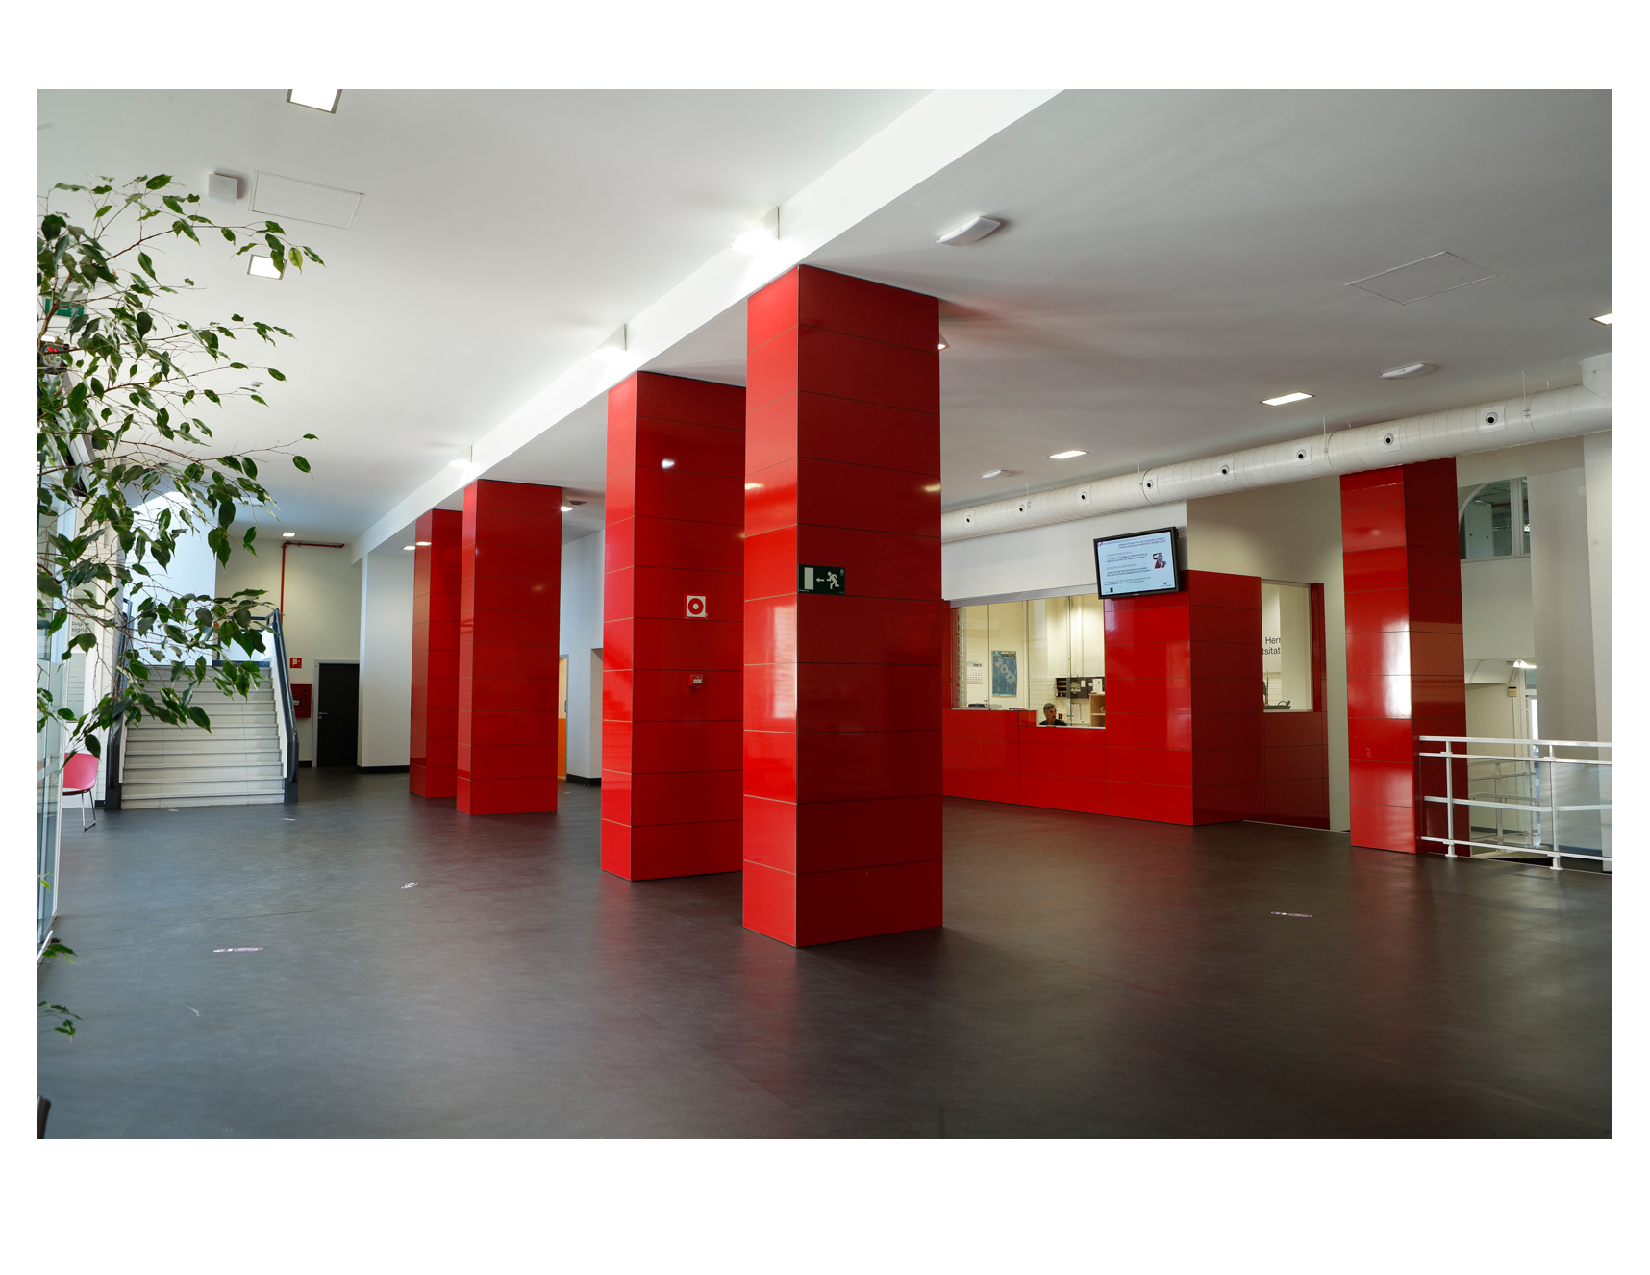
\includegraphics{figs/hall.pdf}} 
    \caption{\emph{Informatika Fakultate}ko sarrera.} 
    \label{fig:infor-sarrera} 
  \end{center} 
\end{figure}

Kodea:
\vspace{0.5 cm}

\begin{minipage}{8cm}
\begin{verbatim}

\begin{figure}[htbp] 
  \begin{center} 
    \scalebox{0.4}{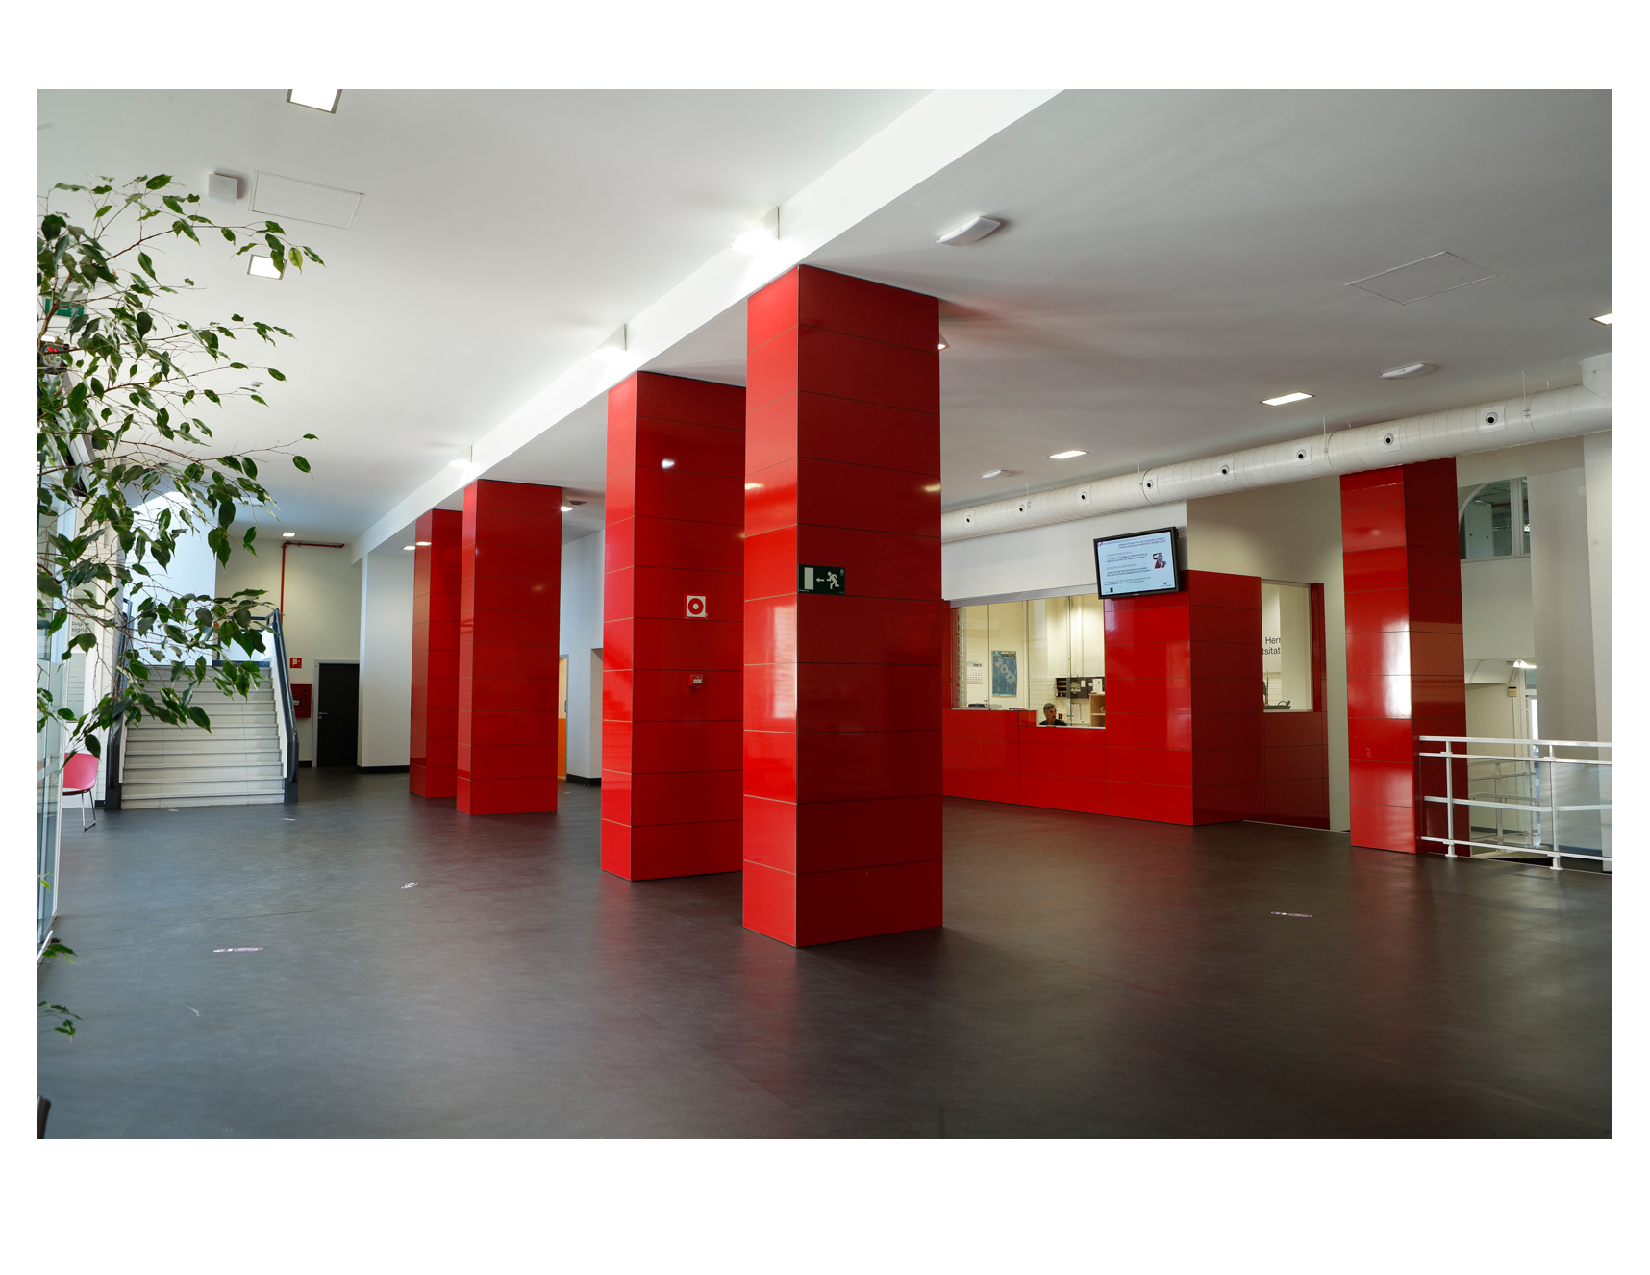
\includegraphics{figs/hall.pdf}} 
    \caption{\emph{Informatika Fakultate}ko sarrera.} 
    \label{fig:infor-sarrera} 
  \end{center} 
\end{figure}

\end{verbatim}
\end{minipage}


\subsection{Letra"-motak}
\label{azpiatala:letra}


Testua bai \textbf{beltzez} (\verb+\textbf{beltzez}+), edo letra \emph{etzanaz} (\verb+\emph{etzanaz}+) edo \textit{italikaz} (\verb+\textit{italika}+) idatz dezakezu. Baita \textsc{hizki"-larri txikietan} (\verb+\textsc{hizki-larri txikietan}+) ere.


Gainera hizkiaren tamaina alda dezakezu:

\begin{itemize}
 \item {\tiny honela}(\verb+{\tiny honela}+)
 \item {\scriptsize honela} (\verb+{\scriptsize honela}+)
 \item {\footnotesize honela} (\verb+{\footnotesize honela}+)
 \item {\small honela} (\verb+{\small honela}+)
 \item {\normalsize honela} (\verb+{\normalsize honela}+)
 \item {\large honela} (\verb+{\large honela}+)
 \item {\Large honela} (\verb+{\Large honela}+)
 \item {\LARGE honela} (\verb+{\LARGE honela}+)
 \item {\huge honela} (\verb+{\huge honela}+)
 \item {\Huge honela} (\verb+{\Huge honela}+)
 \item \ldots 
\end{itemize}


\subsection{Bibliografia}
\label{azpiatala:biblio}

Bibliografia oso modu egokian lantzen da \LaTeX{}"-en. Liburu, artikulu edo web"-orrien erreferentziak aparteko fitxategi batean biltegiratzen dira.

Adibide honetan ``main.tex''-en arabera erreferentziak \emph{bibliografia} izeneko fitxategian (\verb+\bibliography{bibliografia}+), biltegiratuta daude honako moduan:
 
\vspace{0.25 cm}

Kodea:
\vspace{0.25 cm}

\begin{minipage}{8cm}
\begin{verbatim}
@book{DBLP:books/aw/Lamport86,
	author    = {Leslie Lamport},
	title     = {LaTeX: User's Guide {\&} Reference Manual},
	publisher = {Addison-Wesley},
	year      = {1986},
	isbn      = {0-201-15790-X},
	bibsource = {DBLP, http://dblp.uni-trier.de}
}
\end{verbatim}
\end{minipage}

\vspace{0.25 cm}

Gero, testuan aipamena egiteko, adibidez, (\cite{DBLP:books/aw/Lamport86}), zera idatzi behar da: \verb+\citep{DBLP:books/aw/Lamport86}+.

Testuaren barruan erreferentzia egiteko, adibidez, \cite{DBLP:books/aw/Lamport86}-ren arabera honako modua erabili behar duzu:  

\verb+\cite{DBLP:books/aw/Lamport86}+.


\subsection{Footnotes}
\label{azpiatala:oin-oharrak}

Footnote edo oin"-oharrak\footnote{Adibide moduan ohar txiki bat.} \verb+\footnote{}+ aginduaz ipintzen dira.



\section{Erderetako terminoen itzulpena}
\label{azpiatala:erdarak}

Orokorrean, bestelako hizkuntzetatik itzulitako terminoak, ingelesetik adibidez, letra"-etzanez idatziko dira. Adibidez, \emph{on"-line}, \emph{wrapper}, \emph{proxy} \ldots


% Ondorengo lerroak ipinita, fitxategi hontatik bertatik konpilatu ahal izango duzu dokumentua


%%% Local Variables: 
%%% mode: latex
%%% TeX-master: "../NAGUSIA"
%%% End: 





















% line in order to check if utf-8 is properly configured: áéíóúñ

\else
\chapter{Ciclo de vida y Participación de los usuarios en el proyecto}
\label{ch:ciclo de vida}


% El siguiente es el texto que aparece en el encabezamiento del proyecto fin de grado (si se quiere que sea distinto al nombre del capítulo))
%\chaptermark{PFG}

En este capitulo vamos a hablar sobre los ciclos de vida del proyecto y la participación de los usuarios dentro de los mismos.

\section{Ciclos de Baldugenda}
\label{secc:ciclos de Baldugenda}

En este apartado vamos a explicar el ciclo de vida y la participación de los usuarios. 

El principal riesgo es que Baldugenda no resulte atractiva para los usuarios. En el desarrollo de proyectos dirigido a móviles en los que el desarrollador no tiene experiencia previa y es un proyecto pensado por él, suele suceder que el proyecto se realice con fallos de diseño o con funcionalidades que los usuarios no ven necesarias. Estos mismos usuarios echan en falta funcionalidades que sí que hubieran incluido si se les hubiera pedido opinión. 
Por este motivo, se trabajó con usuarios durante los tres ciclos de vida que tiene Baldugenda.

El modelo de ciclo de vida que se decidió usar en el proyecto fue el siguiente, un modelo de ciclo de vida de desarrollo en espiral, se realizaron 3 ciclos principales en los cuales se iban añadiendo nuevos usuarios.
Si se quiere entender un poco más este concepto de ciclo de vida en espiral, primero hay que comprender de qué trata. Si se compara con el desarrollo de un modelo en cascada, se puede ver que mientras en el modelo en cascada primero se buscan los requisitos, después se diseña la aplicación, se implementa y ya para finalizar se realizan las pruebas y el mantenimiento. 
En espiral primero se determinan objetivos que se quiere alcanzar en ese ciclo, tanto requisitos, como restricciones. Después se desarrolla la aplicación y se realizan las pruebas y una vez realizadas esas pruebas, se planifica lo que se va a realizar para el siguiente ciclo y lo que se dejara fuera del proyecto. 

\begin{figure}[H] 
  \begin{center} 
    \scalebox{1}{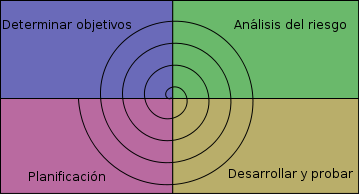
\includegraphics{figs/Espiral.png}} 
    \caption{Desarrollo en Espiral Wikipedia} 
    \label{fig:Espiral} 
  \end{center} 
\end{figure}

Durante cada uno de los ciclo se determinaba un alcance y unas pruebas concretas.Ahora procederemos a explicar cada uno de los ciclos seguidos durante el proyecto.

% Please add the following required packages to your document preamble:
% \usepackage{booktabs}
% \usepackage{graphicx}
\begin{table}[h]
\centering
\resizebox{\textwidth}{!}{%
\begin{tabular}{@{}ccccc@{}}
\toprule
Ciclos  & \multicolumn{1}{l}{Nº personas} & Objetivos                                                                                                                              & Riesgos                                                                               & Desarrollo                                                                                           \\ \midrule
Ciclo 1 & 2                               & \begin{tabular}[c]{@{}c@{}}Casos de uso básicos \\ (Exámenes, Asignaturas)\\ API Google Calendar\\ Corrección  de errores\end{tabular} & API Google Calendar                                                                   & Objetivos implementados                                                                              \\ \midrule
Ciclo 2 & 6                               & \begin{tabular}[c]{@{}c@{}}Modificaciones y Borrados\\ (Exámenes, Asignaturas)\\ Notas\\ Corrección de errores\end{tabular}            & \begin{tabular}[c]{@{}c@{}}Dos tipos de BD distintas\\ en funcionamiento\end{tabular} & \begin{tabular}[c]{@{}c@{}}Conversión de la BD\\ implementada\\ Objetivos implementados\end{tabular} \\ \midrule
Ciclo 3 & 15                              & \begin{tabular}[c]{@{}c@{}}Backup\\ Descripción examen\\ Modificaciones App\\ Corrección de errores\end{tabular}                       & API Google Drive                                                                      & Objetivos implementados                                                                              \\ \bottomrule
\end{tabular}
}
\caption{Resumen Ciclo de Vida}
\end{table}
 
\subsection{Ciclo Uno}
\label{subsecc:ciclo Uno}

Para este ciclo los Baldusers que estaban dentro del proyecto eran el tutor y el desarrollador de la aplicación. Las funcionalidades que se decidieron para este primer ciclo fueron los casos básicos referentes a la creación de asignaturas y exámenes, dentro de estos casos básicos podemos encontrar la creación de una asignatura con una lista de enlaces y la selección del tipo de evaluación que tiene la asignatura. En cuanto a los exámenes, la creación de exámenes asociados a una asignatura con una fecha en concreto y la hora en la que se realizaría el examen.
También se decidió incluir el API de Google Calendar al proyecto, y con el API se incluyeron más funcionalidades, la creación de un evento, dentro de un calendario de Google Calendar propiedad del usuario como recordatorio del examen. El usuario podría escoger si quiere notificaciones en ese evento o no, se agregó la  posibilidad de modificar los calendarios de Google propios del usuario dentro de la aplicación, y poder añadir o borrar calendarios existentes.
 
Dentro del ciclo aparte del alcance hubo una parte de pruebas donde el tutor y yo usaríamos Baldugenda y comprobaríamos que funcionaba correctamente para proceder a pasar al ciclo dos.


\subsection{Ciclo Dos}
\label{subsecc:ciclo Dos}

Después de realizar el ciclo uno, se revisaron las funcionalidades propuestas e implementadas durante el primer ciclo. A la hora de realizar esta revisión se separaron las propuestas en 3 bloques, uno para las funcionalidades que se mantendrían o se implementarían durante este segundo ciclo, en el segundo bloque estarían las funcionalidades que o por falta de tiempo o complejidad se dejarían para ciclos siguientes y en el bloque tres estarían las funcionalidades que quedarían fuera del proyecto porque se alejaban mucho de la idea inicial o por el coste que supondría hacerlas.
Las funcionalidades que se decidieron mantener del primer ciclo fueron la mayoría de las funcionalidades, ya que al ser el primer ciclo, eran funcionalidades muy básicas como para poder desecharlas. Las implementaciones que se realizaron pero que no convencieron a los Baldusers de ese ciclo, se quitaron para el siguiente y se decidió que si en el futuro hubiera tiempo se volverían a incluir. Una de las funcionalidades que sufrió este cambio fue la de las notificaciones en los exámenes mediante Google Calendar. Durante el ciclo uno se implementó para ver su funcionamiento pero no convenció a los Baldusers y se retiró para el comienzo del ciclo dos.

Para el alcance de este ciclo, los Baldusers agregados, probaron Baldugenda, y devolvieron el feedback sobre la aplicación que había resultado del ciclo uno. Dentro de este feedback se les pidió que dijeran funcionalidades nuevas que podrían añadirse en Baldugenda. Surgieron bastantes funcionalidades, como pasó en el ciclo uno se volvió a dividir esas funcionalidades en 3 bloques y durante la fase para determinar los objetivos se escogió que funcionalidades se realizarían en este ciclo.
Para disponer de la información que devolvían los Baldusers de una manera rápida se decidió usar documentos de Google Drive y compartirlos a los Baldusers, ellos mismos irían rellenando lo que querían agregar a la aplicación y después en la fase de toma de decisiones se escogería que se dejaba fuera.

En el bloque de los casos de uso que se realizarían durante este ciclo se agregó que los usuarios pudieran modificar una asignatura o un examen. Por otro lado también se decidió implementar el que el usuario pudiese borrar las asignaturas que no tuvieran exámenes asociados. Como aspectos nuevos que se incluirían en el ciclo dos fueron, añadir nota en examen y en asignatura. Como también solucionar los errores encontrados por los Baldusers cuando estaban realizando las pruebas.

En el apartado de diseño los Baldusers se quejaron y ellos mismos propusieron un diseño que les parecía más atractivo.
Hubo casos de uso y aspectos que se tuvieron que dejar fuera como fue el caso de agregar nuevos eventos como, las tutorías o los trabajos grupales e individuales.
Las funcionalidades que los Baldusers sugirieron y que nos parecieron interesantes pero se realizarían más adelante fueron, la de agregar descripción en exámenes, y realizar unos ajustes en la aplicación para que cuando se crease un examen o una asignatura mostrara la asignatura o examen directamente sin tener que realizar una búsqueda después.

Durante la fase de análisis de riesgos se tuvo en cuenta que al ser una segunda versión de la aplicación, ya habría Baldusers que se la habían instalado y que en sus dispositivos estaba una versión de base de datos con un esquema distinto del que se lanzaría en la nueva versión, por este motivo lo primero que se llevaría a cabo seria el apartado de realizar una correcta transformación de la base de datos antigua a la nueva sin que los Baldusers perdieran la información almacenada hasta ese momento.

Para la parte de implementación se buscó la manera de que el Balduser que probara la aplicación no se viera afectado con los cambios realizados, para conseguir ese objetivo el único aspecto de diseño que se modifico fue los iconos del menú principal.También a la hora de implementar los nuevos campos de nota en examen y en asignatura, se tenía que tener en cuenta tanto a los Baldusers que habían probado la aplicación como a los que la probarían en un futuro, por eso se tenía que tener en cuenta las dos situaciones que se podían dar cuando los Baldusers probaran la nueva versión. Podía darse el caso que el Balduser fuera nuevo o por el contrario ya la tuviera instalada y solo tuviera que actualizarla.

Para la fase de pruebas se les informo a los Baldusers que ya podían actualizar Baldugenda a la nueva versión con los cambios que habían solicitado. En ese momento los Baldusers tenían que realizar pruebas comprobar el diseño e informar de  cualquier fallo que se produjese en la aplicación. La fase de pruebas era una fase importante en este ciclo, ya que al haber agregado funcionalidades nuevas, tenían que funcionar correctamente si se quería empezar un ciclo nuevo sin problemas. Durante la fase de pruebas no se encontraron fallos importantes, los fallos que se encontraron se pudieron solucionar antes de comenzar el nuevo ciclo.

\subsection{Ciclo Tres}
\label{subsecc:ciclo Tres}

En este ciclo el funcionamiento vario con respecto a los anteriores, hay que recordar que durante el ciclo uno la cantidad de usuarios que podían usar la aplicación era un grupo reducido de 1 o 2 personas, en el ciclo dos el grupo de usuarios paso de ser 2 personas a ser 6 personas, y en el ciclo tres se volvió a aumentar el grupo de Baldusers y se probó con 15 personas.

Para empezar, en este ciclo se les permitió a los Baldusers descargar la aplicación que se había desarrollado hasta el momento en el ciclo dos, y se les pidió el feedback después de que realizaran unas pruebas, se cambió el método de adquirir la información de los Baldusers, ya que nos dimos cuenta que durante el ciclo dos el feedback producido por esos medios no fue suficientemente productivo. Por este motivo se les dio la posibilidad de ponerse en contacto conmigo tanto por teléfono, email o en persona para que me fueran informando de los cambios que veían necesarios para Baldugenda.
En algunos casos cuando el Balduser pudo quedar conmigo se realizaron una serie de pruebas para saber cómo interactuaba el Balduser con la aplicación, una de esas pruebas era la de tener que realizar una serie de acciones con Baldugenda y se le iban contando las pulsaciones que realizaba y el tiempo que le llevaba realizar cada tarea.

Los Baldusers respondieron mejor que la vez pasada aunque hubo más problemas a la hora de instalar la aplicación ya que el tipo de usuario que se escogió fue un tipo de usuario que no tenía conocimientos de informática, esto repercutió en el tiempo que necesitaban para instalarse la aplicación. Del feedback que se recibió de los Baldusers, se incluyó en la implementación de este ciclo el apartado de poder realizar un backup de la información, para después poder recuperarla. También se agregó la descripción dentro de examen, esta funcionalidad estaba presente en el feedback de los usuarios del ciclo dos pero por tiempo no se pudo incluir. La mayoría de las funcionalidades que se modificaron fueron cambios en el funcionamiento en la interacción con la aplicación, cambios del tipo pulsación de los botones o nuevos accesos a los casos de uso ya implementados. Se dejaron casos de uso fuera como fue el caso de modificar todo el diseño de la aplicación que se dejó para los siguientes ciclos.

En la fase de análisis de riesgos se tomó en cuenta que al querer implementar el backup con un servicio de Google, el API de Google Drive,  las dificultades que podían salir a la hora de trabajar con una tecnología que no se conocía de antes, se solventarían atrasando el caso de uso del backup a un ciclo posterior, siempre y cuando esas dificultades produjesen un coste superior al planificado durante el ciclo, si no se consiguiera implementar con la tecnología de Google, se realizarían backups de manera alternativa.

En la fase de implementación se desarrolló con éxito el apartado del backup con unos pequeños problemas al principio, los cuales por medio de documentación oficial se consiguió arreglar. Dentro de la fase de implementación tuvimos en cuenta que en ese momento podían existir 3 versiones de la aplicación, la versión del ciclo uno, la del ciclo dos y la versión actual del ciclo tres, así que había que tener cuidado con esa cuestión ya que la aplicación tenía que seguir funcionando daba igual de que versión se llegara. Cuando se acabó la implementación se subió a Google Play para compartir con los Baldusers la nueva versión, se la descargaron y realizaron unas pruebas para encontrar fallos. Todos los fallos que se fueron encontrando hasta la fecha se fueron resolviendo en una versión nueva cada semana.

Los objetivos que se marcaron para dar conclusión al ciclo tres fueron el de alcanzar una versión estable del producto e implementar las funcionalidades que se habían decidido incluir durante los tres ciclos. A partir del tercer ciclo Baldugenda está recibiendo actualizaciones cuando los Baldusers encuentran fallos se realiza un mantenimiento de la aplicación y se vuelve a subir la nueva version a Google Play . 
\newpage
\section{Participación de los usuarios en el proyecto}
\label{secc:Participación de los usuarios en el proyecto}

Ya se ha ido comentando como dentro de cada ciclo se iba cambiando el numero de Baldusers, las labores que realizaron los Baldusers fueron de distintos ámbitos. Hubo Baldusers que no devolvieron un feedback importante en cuanto a nuevas funcionalidades pero si que fueron reportando cada fallo que se producía en la aplicación. 
Aparte de los feedbacks que iban realizando también se realizaron unas pruebas con alguno de ellos, de estas pruebas se pudieron sacar datos interesantes en cuanto al uso de los usuarios dentro de un proyecto software destinado a móviles, como puede ser la edad o los conocimientos informáticos.

En el capitulo de usuarios se detallara en profundidad el tipo de documentos que se usó para realizar las encuestas y para recoger el feedback. También en este capitulo se podrá encontrar los medios de comunicación usados con los usuarios y problemas encontrados.



% Mediante los siguientes comandos, podrás compilar el conjunto de ficheros desde este mismo documento


%%% Local Variables: 
%%% mode: latex
%%% TeX-master: "../Principal"
%%% End: 


















% line in order to check if utf-8 is properly configured: áéíóúñ
\chapter{Usuarios}
\label{ch:Usuarios}


% El siguiente es el texto que aparece en el encabezamiento del proyecto fin de grado (si se quiere que sea distinto al nombre del capítulo))
\chaptermark{PFG}

El método de trabajo usado en este proyecto se basó totalmente en los usuarios, como método de creación de una aplicación. Las aplicaciones tanto para móviles como para ordenador tienen un público definido y por ello se les tiene que dar importancia a los usuarios.
Hay desarrolladores que realizan el proceso de pruebas con usuarios una vez creados los casos de uso, y utilizan a los usuarios para buscar fallos en su producto. El método que se quiso seguir en este proyecto  es un tanto distinto, utilizando a los usuarios principalmente para facilitar al desarrollador a realizar todas las pruebas sobre la aplicación, pero no es la finalidad principal de estos usuarios. El enfoque que se les dio a los usuarios aquella vez, fue un trabajo más en equipo con el desarrollador.

Los usuarios son los que van a usar la aplicación y los que van a tener que querer descargársela.Si los casos de uso que se implementen no están dirigidos a todo tipo de usuarios, el número de personas que se la descarguen será pequeño.
Por este motivo, los usuarios irán diciendo que casos de uso se incluirán en las siguientes versiones de la aplicación y como la construirían ellos si la fueran a usar día a día.
El método consiste en la implementación de la aplicación por ciclos pequeños que no superen el mes de desarrollo.
Cada ciclo tendrá unos usuarios específicos, y la aplicación ira creciendo y modificándose al cabo de los ciclos, para que al finalizar, en cada ciclo se tenga una aplicación funcional con más casos de uso que la anterior.

Para empezar el primer ciclo, los Baldusers que tomaron parte fueron el tutor y el desarrollador.
En este ciclo se desarrolló la idea y se implementaron casos de uso simples pero funcionales.
Cuando se consiguió un producto enfocado a lo que sería la idea final, se incluyeron 4 personas nuevas. Estas personas debían ser usuarios que el desarrollador supiera que iban a probar su aplicación y se molestarían en responderle a las preguntas sobre la aplicación. 

En este ciclo el desarrollador se puso en contacto con esos usuarios y les hizo llegar la aplicación. Ellos la probarían y le dirían al desarrollador lo que tendría que añadir y modificar de la versión inicial. El desarrollador aparte de escuchar las propuestas les realizó una serie de encuestas para comprobar que tipo de usuarios eran.
Al finalizar el ciclo con los usuarios anteriores se escogieron los casos de uso que se iban a realizar de forma inmediata, los que se realizarían en versiones siguientes o los que se quedarían fuera del proyecto.
Se implementaron los casos elegidos que darían paso a un nuevo ciclo donde se aumentaron el número de usuarios.

En este ciclo el tipo de usuario era muy importante, no importaba tanto la cantidad de personas sino el tipo de persona a las que se metían  para hacer las pruebas.
Se duplicaron el número de usuarios que se había escogido para la anterior y se escogieron de 8 a 10 usuarios nuevos, con distintos tipos de perfil, y se subirá una versión nueva de la aplicación con los cambios realizados.
Hubo que avisar a los usuarios antiguos que se había subido una versión nueva y a los nuevos, se les dio acceso y se les dijo que se la descargaran.
Al finalizar el ciclo se tuvieron casos de uso nuevos de 15 personas distintas que se tuvo que escoger cual se implementaría  y que modificaciones se harían.
Después se realizó una versión nueva y se subió, y los usuarios invitados la testearon para encontrar fallos.



\section{Tipo de usuarios}
\label{secc:tipo de usuarios}

En Baldugenda se han estado usando diferente tipos de usuarios y se ha podido comprobar la diferencia de usar distintos perfiles de personas para desarrollar una aplicación móvil.
Hay distintos ámbitos que separan los perfiles de los usuarios, se pueden dividir por edades, también por tipos de estudios, por conocimientos sobre el tema, o por sexo.
Aparte de esas divisiones hay muchas otras pero en el caso de Baldugenda no se precisó de más para sacar conclusiones.
La mayoría de los usuarios que probaron la aplicación fueron hombres, hubo dos mujeres en la fase de usuarios y las diferencias de la división por sexo no se encontraron, así que no se le dieron importancia en las fases siguientes.
Hay colectivos como los discapacitados que son usuarios especiales a los que hay que desarrollar cosas muy específicas para ellos, por este motivo y porque si se realizaba un trabajo de este estilo hubiera aumentando muchísimo el coste se decidió no incluirlos en las divisiones y añadirlo dentro de las exclusiones del proyecto.
Dos divisiones que sí que se vieron muy afectadas a la hora de hacer las pruebas fueron la de la edad y los conocimientos sobre el tema, en esta situación se hablaban sobre el tema informático y manejo de dispositivos móviles.

Se tuvo que escoger el tipo de usuario que se buscaba que fuera significativo dentro de la aplicación, por ello y viendo el tipo de aplicación que se quería realizar, se decidió que el usuario final debía ser usuarios universitarios, ya que la aplicación tenía como puntos muy específicos las asignaturas y los exámenes, asuntos que van muy ligados al ámbito de los estudiantes.
Esa decisión marco el tipo de usuario que se escogería en las primeras pruebas, las 4 personas primeras eran universitarios todos y no se le dio importancia a sus conocimientos sobre informática ni sobre móviles, lo único que importo fue que tuvieran dispositivos compatibles y que tuviera relación cercana a ellos, para poder tener los resultados lo más pronto posible.

Al realizar las pruebas, se determinó que fue un fallo no tener en cuenta el nivel de conocimiento en informática ya que  este nivel marca mucho la diferencia entre los usuarios a la hora de transmitir las opiniones sobre posibles mejoras.
Un 75\% de los usuarios que se escogieron fueron informáticos y a la hora de devolver el feedback sus respuestas no eran de un usuario común, sino que devolvían las respuestas con una solución que implementaron ellos, aunque ni tan siquiera supieran programar con Android.
Eso fue un problema, ya que no daban casos de uso sino que solo decían de arreglar cosas. Por este motivo se les indico explícitamente  que dieran por lo menos 2 casos de uso nuevos que les parecieran interesantes incluir en una aplicación de este estilo.
De estas ideas salió el añadir las notas a las asignaturas o poder borrar y modificar los exámenes.

Para el segundo ciclo se tuvo que poner un filtro para el tipo de usuario que se buscaba conseguir, ya que en las primeras pruebas se consiguió el ese dato que se tuvo en cuenta para las siguientes y no se agregó tantos usuarios de la facultad de informática y a los que se les incluyo se les dijo especialmente que actuaran sin tener en mente la implementación.
La charla con los Baldusers informáticos surtió efecto solo con la mitad de los nuevos usuarios de informática ya que seguían hablando como si lo fueran a implementar ellos o con un lenguaje técnico que después de muchas frases lo único que pedían era cambiar los colores de un botón. 
Se optó por buscar en distintas facultades, amigos y gente cercana que pudieran probar la aplicación, el mayor problema era que cuanto más se abría el circulo de personas que probaban la aplicación, más difícil era seguirles la pista de lo que hacían. 
Se unió gente de facultades como ADE o Química, una propuesta interesante de mi tutor fue agregar a algún profesor, pero por falta de tiempo al tener que agregar y ayudar a los usuarios que se habían unido en este ciclo no se pudo contactar con ninguno.
Pero ya que no se podía disponer de un profesor, se decidió variar la edad de los Baldusers y comprobar que tal funcionaba la aplicación con ese cambio.

Cuando se decidió agregar a gente de diferente edad y que fuera cercana a mí, sin pensármelo dos veces recurrí a la familia, ellos no pueden decir que no.
El problema fue precisamente que al no poder decir que no, se unieron,  pero alguno no realizó el feedback o no pudieron instalársela por falta de tiempo o conocimiento.
Si hubieran sido los primeros usuarios, hacerles un seguimiento más cercano sí que hubiera sido posible, pero ya habiendo tanta gente metida y teniendo que hablar con cada uno por separado para no contaminar los pensamientos que tienen sobre la aplicación, tuve que optar por mandarles un manual de instalación realizado por mí, y en el caso que no funcionara, decirles que no se preocuparan.

Uno de los familiares era mi madre que tenía el perfil de una mujer adulta con conocimientos mínimos en informática y que sabía manejar el móvil pero a un nivel usuario básico.
Y el otro familiar era mi primo, un adolescente de 16 años que está cursando bachiller, se decidió incluirle aunque fuera una aplicación dirigida especialmente para universitarios, para saber la acogida y el funcionamiento que se le podría dar fuera de la universidad y si se podría o no extrapolar a otras áreas como colegios o institutos.
Durante este ciclo la parte más complicada fue incluir a la gente en el proyecto y conseguir que sé descargaran la aplicación, ya que se había decidido no incluir a gente que tuviera mucho conocimiento de informática, eso aumentaba el tiempo de explicación a la hora de realizar la descarga.
Las fechas en las que se escogió a la gente no fue acertada ya que era principio de exámenes y los Baldusers estaban a mil cosas y no podían realizar el feedback en las fechas señaladas.

A la hora de trabajar con usuarios hay que saber qué tipo de usuarios interesa tener en el proyecto y cuales aportaran más información.
Mucha de las cosas que digan los usuarios hay que filtrarlas y compararlas con su tipo de perfil a la hora de realizarlas, por ejemplo si solo uno de los usuarios se ha quejado de la letra y justo ese usuario es el único que tiene un modelo de móvil de los más viejos posibles, igual no compensa realizar muchas modificaciones que puedan alterar el diseño de los otros usuarios que no se han quejado. Aparte esos usuarios que tienen en este momento un móvil viejo, llegara un punto en el que lo tengan que actualizar por uno más nuevo y llegado ese punto se podrá prescindir de esa actualización de la letra.

Se ha hablado del tema de los usuarios como personas y de sus conocimientos, pero hasta el momento no se le ha dado importancia ni se ha hablado de algo muy importante que afecta a los usuarios, su dispositivo móvil. 
Cada usuario es distinto, aparte de lo mencionado antes, también por el tipo de dispositivo que usan, hay usuarios que tienen móviles con pantallas enormes que no les entra ni en el bolsillo y otros con una pantalla tan pequeña que lo pueden llevar en el bolsillo de la camisa.
Aparte de la pantalla, un aspecto importante es la versión del móvil ya que no es lo mismo un móvil actual con la versión más nueva o un móvil de hace 3 años con una versión muy antigua de Android.
Por eso antes de escoger a los usuarios, hay que tener alguna idea del tipo de dispositivo que usan, por lo menos el tamaño de la pantalla o si disponen de teléfono, de poco serviría un usuario que no disponga de teléfono a menos que solo se necesiten ideas a nivel conceptual.




\section{Pruebas}
\label{secc:pruebas}

A la hora de realizar las pruebas con los Baldusers se decidió seguir una metodología utilizada en la asignatura de Interacción Persona Computador, que consiste en ofrecer unas pautas a seguir al usuario, llevar la cuenta de las pulsaciones que realiza y el tiempo que tarda en realizar las acciones.
Para empezar a realizar las pruebas, un punto importante era conseguir que se descargaran la aplicación.
Fue una tarea dura, ya que Google no permite realizar invitaciones individuales a la aplicación, así que hubo que incluirlos en un grupo y después confiar en que ellos supieran aceptar la invitación e unirse a la fase alpha.

Una vez logrado el objetivo de instalar la aplicación en los dispositivos de los usuarios, la siguiente tarea fue la de pedirles información referente al tipo de usuario que eran, esta información se consiguió mediante unas preguntas realizadas por medio de formularios que rellenarían una vez y con eso se tenía una idea del tipo de perfil que tenía el usuario.
Se les dio una semana para que pudieran realizar las pruebas pertinentes y acostumbrarse a la aplicación, durante esa semana se les pidió que fueran escribiendo el feedback que se les ocurriese en un documento compartido que se les había pasado por medio de la aplicación y de la comunidad de Google.
Algunos lo rellenaron sin poner problemas, otros hablaron directamente conmigo diciéndome el feedback y otros no realizaron ninguna de las dos cosas anteriores.

Para estos últimos usuarios, se tuvo que estar metiendo presión y haciéndoles acordar que se necesitaba el feedback lo antes posible. Ellos solo dieron largas y aportes estéticos, no un feedback consistente como se había preparado en un principio.
Si se querían realizar las modificaciones para la versión siguiente se precisaba de los casos de uso que dijeran los usuarios, por este motivo ya que no decían ningún caso de uso se les mando la tarea de que pensaran casos de uso útiles para la aplicación.
Los Baldusers respondieron positivamente, ya que no se les exigió esta vez escribir en ningún documento, solo se les dijo que me lo comunicaran por el medio que mejor les viniera.
Durante el segundo ciclo de pruebas la cantidad de usuarios aumento y con ello el tiempo que tenía que pasar ayudándoles también.
De lo aprendido en la vez pasada sobre los documentos de feedback con los usuarios y para no estar esperando que escribieran, se les facilito mi número de teléfono y mi correo, para que si se les ocurría algún caso de uso o les daba algún error me lo comunicaran por cualquiera de esos medios. Ya que había confianza con estos usuarios y ser un grupo reducido no importaba usar estos medios de comunicación para leer a cada Balduser ya que se asumía que si en la vez pasada que siendo 4 solo la mitad cumplió correctamente, esta vez solo tendría que hablar como mucho con 5 personas las demás o no me hablarían o si lo hacían serian unas pocas líneas.

Al recibir los mensajes de los Baldusers iba tomando notas de lo que pedía cada uno, y ya que no tenía que esperar a que me lo escribieran podía empezar a darle prioridad y preguntarles directamente a que se referían con aspectos de diseño o como les parecía mejor si una opción u otra.
Esta solución funciono mejor, no era tan profesional como recolectar la información directamente mediante formularios y documentos, pero al hacerlo de esta manera los Baldusers no  se sentían tan obligados a realizar cosas y les daba menos pereza hacerlo, aparte al ser la mayoría universitarios estaban siempre con el Whatsapp o Telegram encendido, medio que usé para relacionarme con ellos lo más rápido posible al saber que ya habían probado la aplicación.

Cuando se producía un error en alguno de los dispositivos de algún Balduser me llegaba al correo electrónico una notificación y todas las líneas de código que habían activado tal error.
De esta forma el tiempo que me ahorraba al preguntar el motivo a cada Balduser se reducía enormemente.
Aprovechando ese tiempo en arreglar los fallos, o investigar cómo y porque se producían.
Hubo situaciones en las que al no bloquearse la aplicación no se guardaba el fallo en Splunk Mint, en esos casos sí que era beneficioso que el Balduser en cuestión se pudiera poner en contacto conmigo para decirme el motivo y cuando se producía el fallo.

Al tener todo funcionando, los casos de uso listos sin fallos, se les propuso a los Baldusers que tuvieran tiempo, a quedar conmigo para realizar algunas pruebas.
Al ser fechas malas cuando se realizaron las pruebas, no muchos pudieron quedar conmigo en persona. A los que sí que pudieron, se les realizo unas pruebas con la aplicación, las pruebas consistían en lo siguiente:
Como primera prueba tenían que crear una asignatura, se les dejaba la aplicación abierta en el menú principal y sin decirles nada se veía como reaccionaban a la tarea que se les había asignado. La tarea era una muy concreta no tenían que pensar que rellenar ni nada, todo lo que se podía realizar en la tarea estaba ya escrito en la pregunta.
Era interesante comprobar que dependiendo del tipo de Balduser que usaba la aplicación entendía los conceptos de manera distinta. Y también la manera de interactuar con la aplicación era totalmente distinta entre unos y otros.

Hubo Baldusers que no estaban acostumbrados a realizar pulsaciones largas sobre objetos y al no haber incluido en el menú dichas acciones se quedaban bloqueados en distintas preguntas.
Por este motivo se decidió modificar el diseño de la aplicación para que fuera más sencillo para el usuario.
También aparte de darles las tareas que tenían que realizar, se llevaba la cuenta de pulsaciones y el tiempo que tardaban en cada tarea.
Las pulsaciones y el tiempo se usó posteriormente para calificar las tareas de más complicadas a menos complicadas dependiendo del número de pulsaciones y del tiempo invertido en realizaras.

Al finalizar el ciclo se volvió a realizar las modificaciones en la aplicación pero ya realizando una aplicación consistente y sin errores, ya no se añadiría nuevos casos de uso y los casos nuevos de uso que dijeron los usuarios, aunque fueron pocos, se incluyeron en el apartado de posibles mejoras.
Una vez comprobado por el desarrollador que las modificaciones y los errores se solucionaban se volvió a subir una nueva versión de la aplicación. En esta ocasión se agregó a un nuevo usuario que se había quedado fuera en la vez pasada, ya que estaba ocupado en esas fechas.
El usuario que se agrego era miembro de Magna SIS ya que durante el proyecto me había puesto en contacto con la empresa para poder hacer uso de uno de sus proyectos ya realizados en el pasado, aunque al final no se pudo usar, se quiso que algún integrante de la empresa formara parte de los Baldusers.

La última fase de pruebas ya no era como las fases anteriores, en esta fase sobre todo se utilizaba para perfilar el producto y comprobar que no hubiera ningún cabo suelto sobre posibles errores o problemas de diseño no testeados durante las versiones anteriores.
Gracias a esta fase de pruebas, se pudieron depurar fallos con algunas modificaciones y sobre todo con el caso de uso de Backup que se agregó como último caso de uso en la aplicación.
Para esta fase de pruebas, se usó una semana para que los Baldusers comprobaran los fallos que se producían con la nueva versión.
Se estuvo revisando cada día el Splunk Mint, comprobando que todo funcionara adecuadamente y se realizó la subida de la nueva versión.
A partir de este punto se repitió el proceso pero solo para solucionar problemas y ya que no se tenía que unir a más usuarios, eso permitía que el tiempo que no se invertía en eso, se pudiera utilizar realizando los arreglos más rápido.



\section{Tipos de documentos usados}
\label{secc:tipos de documentos usados}

Para la recogida de información por parte de los usuarios se empezó a usar documentos de Google Drive, compartiendo a cada Balduser el acceso y permisos de modificación.
Esos documentos eran un formulario donde el usuario respondía una serie de preguntas sobre sí mismo y otras sobre su dispositivo móvil. Y aparte del formulario había documentos de texto que servían para distintos propósitos.
Uno de esos documentos era una explicación de porqué se había decidido realizar la aplicación y los usos que tenía en esa versión.
Otro documento era un manual donde se les explicaba a los Baldusers como poder instalarse la aplicación si se habían registrado por medio de Google plus.
Y 2 documentos donde los Baldusers escribían el feedback.
Se comprobó que el uso que daban los usuarios a esos documentos no era tan ágil como se pensaba, por ese motivo se decidió cambiar la forma de recoger esa información.
Se empezó a pedir a los nuevos usuarios la información por medio de emails o mensajes entre móviles. Y yo personalmente los redactaba en los ficheros antes mencionados o tomaba apuntes de las modificaciones que se tenían que realizar.
En el caso que las modificaciones no estuvieran claras el tener contacto directo con el usuario me permitía preguntarle el motivo de la modificación y entender porque se había llegado a esa decisión.


\section{Medios de comunicación}
\label{secc:medios de comunicación}

Un punto importante y sumamente necesario a la hora de trabajar con los Baldusers fue le medios de comunicación que teníamos para intercambiar información.
Era muy importante escoger el medio de comunicación antes de empezar a agregar a alguien al proyecto y tener bien claro el tipo de usuario con el que estaría hablando, no era lo mismo invitar a una persona mayor a probar la aplicación, que justo sabe usar el móvil para llamar que a estudiantes de universidad que siempre llevan el móvil en las manos.
Por esos motivos se decidió hacer que el medio de comunicación fuera de la forma más ágil posible.

Al principio se le quiso dar un toque más profesional al realizar formularios y documentos donde los Baldusers tenían que realizar el feedback, pero no funciono así que se optó por el uso de los móviles como canal de comunicación.
Aparte de usar el móvil como canal de comunicación por medio de Whatsapp o Telegram en algún caso, se siguió usando Google Drive para compartir el manual de instalación y los grupos de Google para enviar mensajes grupales.
Al primer grupo de Baldusers se les creo un grupo de Whatsapp para que compartieran por ahí sus dudas con respecto a cómo instalar la aplicación. Pero no resulto como se esperaba, al no conocerse la gente no hablaba por el grupo y el grupo murió pocos días después de crearse.
Por ese motivo, a los siguientes grupos que fueron entrando se les agregó a la comunidad de Google y se les iba informando por ahí o directamente por correo o por Whatsapp.

Un buen método para intercambiar información con los usuarios,  es quedar con ellos en persona, aunque suponga más trabajo y pérdida de tiempo por tener que encontrar un rato que los dos podamos quedar, de esta forma no hay dudas con lo que el usuario quiere.
Cosas como malentendidos o diferentes puntos de vista al ver una función se pueden solucionar mejor si se hablan las cosas a la cara que haciéndolo a través del teléfono.
Por este motivo cuando era crucial saber lo que querían los usuarios o para tomar los tiempos se decidió quedar en vez de decirles a los propios usuarios que se tomaran los tiempos de realización.



\section{Aportaciones Realizadas}
\label{secc:aportaciones Realizadas}

La mayoría de los Baldusers aportaron grandes ideas al proyecto ya que hay muchas funcionalidades, que si no hubiera sido por ellos se hubiera pasado por alto que eran necesarias, por ejemplo la descripción en la parte de los exámenes, no se había tenido en cuenta en un principio, pero después de que uno de los usuarios lo comentara, sí que se le vio utilidad.
En el tema de los errores los Baldusers fueron de gran utilidad, ya que ellos fueron los que descubrieron la mayor parte de los errores dentro de la aplicación, al usar día a día surgen situaciones que no son habituales, como que te llamen por teléfono mientras esta la aplicación abierta o situaciones parecidas, en esas situaciones uno no piensa cuando está implementando el código.
Los aportes que reportaba cada usuario se iban apuntando en un fichero de texto y cuando concluía el periodo de prueba, se solucionaban los errores más grandes que se habían producido, ya que algunos de los casos de uso implementados que daban error, puede que en la siguiente iteración no fueran necesarios.


\section{Usuarios y su relación con las aplicaciones móviles}
\label{secc:usuarios y su relación con las aplicaciones móviles}

Cada vez es más frecuente ver por la calle a todo el mundo con un móvil en las manos, cada persona está acostumbrada a usar las aplicaciones que más le gustan, pero hay aplicaciones que la sociedad las tiene como costumbre. Se han metido tanto en nuestro día a día que no se puede vivir sin ellas. Aplicaciones de mensajería instantánea como son Whatsapp o Telegram son comunes en cualquier dispositivo móvil, han sustituido a las llamadas y los mensajes por la facilidad, rapidez y bajo coste que les supone a los usuarios.
Además de eso, el acceso a Internet está al alcance de la mano de cualquiera mediante los navegadores móviles.

Google tiene un gran monopolio de las aplicaciones más usadas por los usuarios, todos los dispositivos tienen los servicios de Google instalados lo que hace que por defecto ya se tenga preinstalado antes de usar el móvil, Youtube, Gmail, Calendar, Drive y muchos servicios más de Google.
Todas estas aplicaciones son populares por un motivo, porque sirven para que las personas nos relacionemos unas con otras, y Google lo ha conseguido sin lugar a dudas por medio de sus aplicaciones, no hay aplicación de Google que no tenga la función de compartir.
Aparte de esto, como es una familia de aplicaciones, cada una de estas está de alguna forma asociadas con sus hermanas, ya sea porque dan posibilidad de subir un fichero a esa aplicación o dan permiso para compartir a los usuarios de tu correo electrónico.

Los Baldusers que probaron la aplicación eran usuarios de todo este tipo de aplicaciones. Tenían los diseños de estas aplicaciones metidos en la cabeza y también sus funcionalidades, un problema para ser un desarrollador compitiendo contra por ejemplo la empresa de Google.
La mayoría pedían lo que habían visto en otros sitios y como el mercado está lleno de aplicaciones con mucha inversión y parece sencillo su uso, las proponen como casos de uso. 
El problema de ese tipo de situaciones es como decirles a los usuarios que no puedes desarrollar eso, ya que no tienes las herramientas o directamente te pueden denunciar por plagio.
Pero no lo entenderán y seguirán queriendo que se les haga un Calendar con otro nombre pero las mismas funciones.


\section{Problemas encontrados con los usuarios}
\label{secc:problemas encontrados con los usuarios}

Uno de los problemas encontrados al trabajar con usuarios, es la cantidad de tiempo que se gasta al tener que hablar con ellos y explicarles cómo funciona cada cosa.
Lo habitual es que los usuarios pregunten dudas, el desarrollador les resuelve las dudas y para no molestar más al desarrollador, dicen que lo han entendido aunque no sea así, al cabo del tiempo volverán a preguntar la misma duda. Por este motivo es más cómodo  realizar manuales de uso para las preguntas más comunes o para la fase de instalación.

Un tema muy importante si se va a trabajar con usuarios es definir los usuarios antes, y que tipo de respuestas se quiere recibir de ellos. Si se quiere respuestas útiles a la hora de desarrollar la aplicación, hay que escoger bien al tipo de usuario.
Los usuarios cuando devuelven un feedback suelen comparar con aplicaciones ya existentes.
Los usuarios informáticos hablaban como si fuera una aplicación web, los que no eran informáticos la comparaban con cualquier aplicación que han visto parecida o directamente pedían que hiciera magia y convirtiese  una agenda de estudiantes en un secretario personal que les llevase los apuntes al día y les hiciera los trabajos.

En el apartado de la interacción de los usuarios con las aplicaciones móviles ya se ha hablado de los problemas que nos encontramos al ser un desarrollador frente a grandes compañías, por eso mismo hay que tener claro desde un principio lo que se quiere realizar y por mucho que se trabaje con usuarios la meta es clara y el desarrollador es el que tiene que llevar el rumbo de la aplicación adelante. Es correcto que los usuarios pidan lo que han visto que hay por Internet, lo que han probado y les ha gustado, pero igual lo que ellos han probado y que lo usaran igual 1 o 2 veces a la semana, al final el que lo tiene que desarrollar tiene que invertir meses en conseguir un trabajo parecido y ya teniendo en la cabeza que no resultara igual un trabajo que ha realizado una persona frente al que ha realizado un equipo de 100 personas.


% Mediante los siguientes comandos, podrás compilar el conjunto de ficheros desde este mismo documento


%%% Local Variables: 
%%% mode: latex
%%% TeX-master: "../Principal"
%%% End: 


















% line in order to check if utf-8 is properly configured: áéíóúñ
\input{54-aplicación-es}
\chapter{Desarrollo de apps tipo Baldugenda}
\label{ch:desarrollo}

El capitulo de desarrollo de apps tipo Baldugenda se ha dividido en dos partes, una referente a Google y la importancia que tiene en las aplicaciones Android y otra parte donde se hablara mas sobre los aspectos importantes referente al mundo Android dentro del tipo de aplicación que se esta desarrollando, como podría ser el uso de calendarios o las notificaciones.

% El siguiente es el texto que aparece en el encabezamiento del proyecto fin de grado (si se quiere que sea distinto al nombre del capítulo))
%\chaptermark{PFG}


\section{Google}
\label{secc:google}

Un punto importante en lo que al desarrollo de aplicaciones móviles se refiere, es el uso que los usuarios dan a las aplicaciones, hay muchas aplicaciones en el mercado de la tecnología móvil, pero las aplicaciones punteras que salen adelante son las que tiene compatibilidad con otras aplicaciones que usan habitualmente los usuarios como puede ser el correo, las redes sociales, o sin necesidad de ese tipo de funcionalidades, las usan porque son realmente originales en su ámbito.
Google ha hecho un negocio de las aplicaciones y facilita a los desarrolladores a que  realicen aplicaciones proporcionando APIs de sus productos y permitiendo que suban las aplicaciones a su tienda.
En este apartado se detallará el uso de Google dentro de aplicaciones del tipo de aplicación que es Baldugenda, una aplicación que controla calendarios, realiza backups de información  y tiene control de cuentas de Google.

\subsection{Google Play}
\label{subsecc:Google Play}

Para empezar Google proporciona la posibilidad de compartir  las aplicaciones por medio de Google Play.

Para poder desarrollar aplicaciones y colgarlas en el Play Store hay que realizar un pago de 25\$, con ese pago se consigue que la cuenta de Gmail escogida pase a ser de desarrollador, lo que permite crear aplicaciones y subirlas, también se puede monetizar esas aplicaciones por medio de publicidad.

Una vez se ha realizado el pago la creación de una aplicación se separa en dos partes principales.

\begin{itemize}
\item Desarrollo mediante Eclipse o \gls{Android Studio}
\item Subida al Google Play
\end{itemize}

Para programar en Android la mejor opción es la de Android Studio, ya que genera los ficheros y el manifest del proyecto sin tener que estar modificándolo todo el rato.
Si se escoge la opción de Eclipse ya Google no da el soporte necesario y es más complicado programar en él.
Dentro de Android Studio hay varias posibilidades a la hora de crear un proyecto y depende de cuál se escoja funcionara para distintos dispositivos.
Cuando se ha creado el proyecto y se ha conseguido probar sin errores hay que firmar el apk, para esto Android Studio permite generar un apk firmada de una manera fácil.

\newpage
\begin{figure}[H] 
  \begin{center} 
    \scalebox{1}{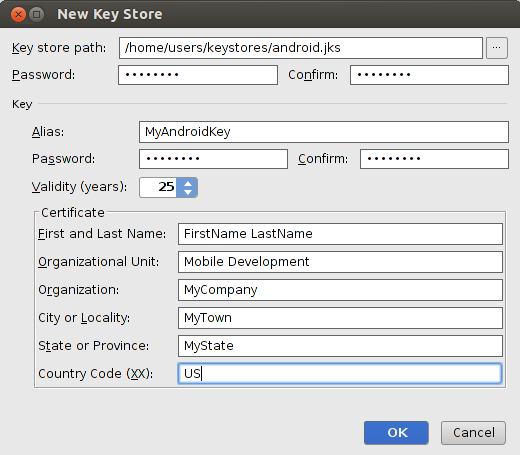
\includegraphics{figs/CreacionKey.png}} 
    \caption{Ventana de creación de Key} 
    \label{fig:CreaciónKey} 
  \end{center} 
\end{figure}

Con la ventana anterior se genera un fichero que se usará como llave para firmar la aplicación, en el caso de necesitar usar APIs de google se necesitará de la contraseña cifrada en Sha1 para enlazar el API con la aplicación.


La parte más pesada después de desarrollar la aplicación es el papeleo con Google, para subir cualquier aplicación hay que rellenar muchos campos dentro del formulario para que Google permita subir la aplicación. Estos campos la mayoría son información de la aplicación como imágenes del icono que usaremos, el tipo de aplicación que es, qué tipo de gente puede usarla, y otras preguntas parecidas a las anteriores.

Una vez Google permita colgar la apk, dará 3 opciones,  en producción, beta  o alfa. Estas opciones limitaran la cantidad de gente que se puede descargar la aplicación. Y ayuda a tener una versión de la aplicación funcionando mientras se está probando una versión superior en otro tipo de subida.
Si se quiere compartir en alpha o en beta hay 2 opciones para agregar a mucha gente a la vez, la primera opción es la que se usó durante la primera fase de las pruebas con los Baldusers, que es creando una comunidad de Google plus y dentro poniéndoles el link para que se la descargasen. O la segunda opción que se usó en la segunda fase de las pruebas, que se creó un grupo de Google groups y se añadió los emails de la gente y dentro de la invitación se les añadió el link de descarga, se limitó los permisos de la gente del grupo para que no pudieran crear nada ni responder a nadie.

La primera opción dio muchos fallos ya que había gente que por el tipo de cuenta que usaban en su universidad o instituto no se les permitía usar Google plus así que no podían asociarse al grupo de usuarios por esa forma, aparte si no se tenía cuenta en Google plus, esta opción les obligaba a crearse cuenta con el coste de tener que explicarles paso a paso como hacerlo si no eran muy entendidos de las redes sociales.
La segunda opción y en mi opinión la más útil fue la de crear los grupos mediante Google Groups, el Balduser solo recibía un email con 2 links, uno para aceptar la invitación y otro para unirse a las pruebas de la descarga de la aplicación. No tenían que hacer nada más. Lo bueno de esta opción es que se estaba trabajando con el grupo de Baldusers como si fuera una lista de emails y en el caso de tener que mandar una información general solo había que redactar un correo de grupo.

Una vez seleccionado los grupos que tenían acceso a la aplicación en fase alpha el siguiente paso era subir la apk.
La subida a Google play no es inmediata, por esta razón cuando se subía Baldugenda solían pasar un par de horas hasta que la descarga estuviera disponible.
Unos puntos importantes a la hora de generar las aplicaciones son el peso de la aplicación, los dispositivos a los que va dirigido y los permisos que se pedirán a los usuarios.
Los dos primeros puntos están vinculados, ya que si se escoge un grupo muy amplio de dispositivos tanto por pantalla como por versión de Android, se estará ante una situación en la que para que se vea correctamente en todos los dispositivos habrá que meter iconos de diferentes tamaños y generar vistas dependiendo del dispositivo.

Siempre hay que pensar que no es lo mismo desarrollar una aplicación web que una aplicación móvil, los dispositivos móviles no disponen de mucha capacidad de almacenamiento así que cuanto menos pese la aplicación, más posibilidades hay de que no de problemas para a la hora de instalarla.
Aparte de los iconos y las vistas también dependemos de las librerías cuanto más alta es la versión de Android más peso añade al programa a la hora de la instalación porque le añade funciones nueva de las librerías aunque no las hayamos usado, como puede ser un cambio de color al pulsar un botón, que aunque en nuestro código no se pueda ver, ni en las versiones anteriores se vea, cuanto mayor es la API más funciones agrega.
Google limita el peso de las apk que se pueden subir a Google Play en 50 mb, a partir de ese peso se pueden subir extensiones para la aplicación.

\subsection{Uso de APIs}
\label{subsecc:Uso de APIs}

Ya se ha explicado cómo funciona la subida de una aplicación a Google play, pero eso no es lo único que Google proporciona de ayuda a la hora de desarrollar la aplicación y distribuirla.
Google proporciona sus APIs propias para que se vinculen los servicios que ofrece Google con la aplicación que se quiera desarrollar. Si la aplicación que se quiere desarrollar no va a realizar un gran uso de los servicios de Google no hay problema, el problema surge cuando se alcanza el límite de usos de la API y Google exige pagos para seguir usándolo al mismo rendimiento.
Aunque a priori las cuotas parecen altas siendo como es el caso de Google Calendar API \cite{GCalendar} de 1.000.000 de solicitudes por día, si una aplicación se quisiera comercializar ya habría que estar al tanto de cuantas solicitudes se realizan y si se necesita aumentar la cuota, puesto que al tener publica la aplicación, cualquiera en el mundo podria descargarsela.

Para el uso de estas APIs, Google ofrece distintas posibilidades dependiendo de la API, ya que hay algunas que necesitan autenticación para funcionar como puede ser el caso de Google Calendar frente a otras como Google maps que lo único que necesitan es la credencial de tu aplicación para llevar al día la cuota de la API.
Este apartado de credenciales de las APIs es un tema bastante difícil a la hora de usar los servicios de Google y donde más problemas se suelen tener. Google lo explica en su web paso a paso como configurar las credenciales. Aunque bastantes veces habrá que generar credenciales que no se sabe para qué sirven porque las que dice Google que se generen no dan acceso a la API.

Dentro de la consola de desarrollador de Google es donde hay que añadir los certificados del API, hay distintas pestañas, algunas dan información del uso que se ha dado del servicio y otras dan la posibilidad de agregar más servicios al proyecto.
Se pueden encontrar servicios tales como el Google Calendar o el Drive que se han usado para la parte de la administración de calendarios y el backup dentro de Baldugenda, como también podemos encontrar servicios de youtube, traductor, publicidad, mapas. 

Todos los productos que Google quiere vender al alcance de los desarrolladores.
Lo bueno que tiene usar los servicios de Google es que todo aquel que se descargue la aplicación habrá usado alguna vez esos servicios o tenga la aplicación instalada en su dispositivo aunque no la use. Si se usaran servicios de terceros que no fuera Google se tendría que pedir al usuario que se creara otra cuenta o que se instalara otra aplicación para poder sacar todo el partido a la aplicación que se está creando.

La finalidad de usar servicios de terceros de empresas importantes en los dispositivos móviles es, que los usuarios usen el producto que se ha desarrollado y que no se lo desinstalen, uno de los motivos por los que la gente desinstala aplicaciones pequeñas es que les exigen estar duplicando información que quieren tener centralizada. Un ejemplo podría ser los eventos del calendario, hay muchas aplicaciones que usan el calendario del móvil pero que no dan soporte a calendarios online como el de Google Calendar, en este caso si el usuario quiere crear un evento con esa aplicación no puede modificarlo desde el ordenador y le limita a usar siempre el móvil con ese evento.
Pasa lo mismo con las notas o con los ficheros al querer guardarlos en los móviles, generando así una necesidad para el usuario de tener un espacio de almacenamiento enorme si quiere sacar fotos y descargase cualquier cosa al móvil.

\subsection{Uso de calendarios}
\label{subsecc:Uso de calendarios}

En el apartado anterior se ha hablado de las APIs,  una de las que proporciona Google es la de Google Calendar, en las aplicaciones parecidas a Baldugenda el uso de Google Calendar no es habitual la mayoría generan los horarios en calendarios propios de la aplicación y te muestran fechas del calendario solo accesibles desde el móvil.
Google al proporcionar el API de Google Calendar y al estar tan vinculado a Android para descargar las aplicaciones proporciona una relación con el calendario del móvil casi perfecta tanto para visualizar los eventos como con las notificaciones de dichos eventos.
Con el servicio del calendario Google permite realizar todo lo que se podría hacer desde el servicio web de Google Calendar pero desde la aplicación que creemos.

A la hora de desarrollar una aplicación usando este API, Google propone 2 formas para empezar a desarrollar, una usando el API Rest y la otra usando la librería java que nos proporcionan con los métodos.
El problema en esta parte es que si se tiene algún problema con el API Rest el código que dan de ejemplo es demasiado pequeño si se quiere realizar cosas complejas. Y en el código de ejemplo que Google tiene en \gls{Github} solo se encuentra el API usando la librería.
Tanto si se usa la librería o si se decide uno por usar Rest, Google ha separado las funciones en apartados para que sea lo más cómodo posible encontrar lo que se necesita.

Algo importante que hay que saber a la hora de programar con este API es que se necesita credenciales OAuth2 y credenciales públicas para que den permiso a la aplicación que se desarrolle a que use el API de Google Calendar.
En el apartado anterior se ha explicado como añadir credenciales al proyecto, una vez añadidas lo que queda es ver que funciones se necesita usar para crear el evento o para visualizar los calendarios y ya se podrá realizar modificaciones en los calendarios de Google.

Cada API es un mundo y este API no se queda atrás, las principales funciones que todo usuario habitual usa, como crear un evento, visualizar los calendarios, etc… son sencillas de usar, el problema surge cuando se empieza a complicar el caso de uso y el uso del API resulta engorroso.
En el caso de Baldugenda se mantuvo el apartado para la gestión de calendarios que proporcionaba Google ya que servía al usuario para crear calendarios específicos para los eventos de la aplicación. Pero dio problemas al no sincronizarse automáticamente al calendario del dispositivo, siendo ese el motivo por el cual muchos usuarios pensaron que no se creaba bien el evento y cuando se ponían en contacto conmigo y se les explicaba como actualizar el calendario les salían todos los eventos e incluso duplicados porque habían generado 2 o 3 exámenes con distinto nombre pero haciendo referencia al mismo examen.

\subsection{Debugging}
\label{subsecc:Debugging}

El apartado de debugging es un punto importante en todo proceso de desarrollo de aplicaciones tanto de móviles como de cualquier otro tipo, pero en el caso de los móviles se vuelve un trabajo muy difícil de llevar a cabo cuando ya está en prueba por usuarios, ya que las los errores que se produzcan no los podrá ver el desarrollador a menos que la aplicación tenga implementado funciones para esos casos.
Cuando se está desarrollando la aplicación, Google proporciona mediante Android Studio una excelente ventana de debugging para seguir paso a paso y  línea por línea el recorrido que realiza la aplicación.
Se puede añadir líneas de log especificando si es de error de peligro o directamente de información. 

Aparte de estos logs se puede seguir el valor que tiene una variable en todo momento desde que nace hasta que muere con la actividad.
El problema de esta forma de debugging es que cuando la aplicación deja de estar conectada al ordenador y al Android Studio, ya no podemos seguir la pista de lo que pasa.
Google proporciona información de los usuarios que se han instalado la aplicación en la ventana donde se ha tenido que publicar dicha aplicación. Aunque esta información es mínima incluye información útil como las versiones de los dispositivos que se la han instalado, la operadora del dispositivo, el país desde donde se la han descargado y el lenguaje de la instalación del dispositivo.
\newpage
\begin{figure}[H] 
  \begin{center} 
    \scalebox{1}{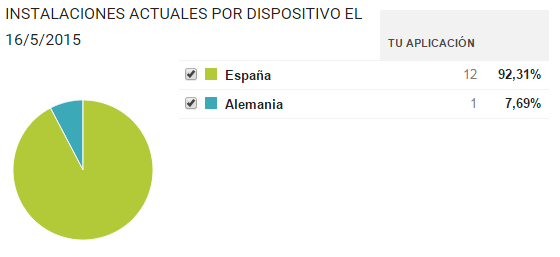
\includegraphics{figs/UsoPorPaises.png}} 
    \caption{Uso por Países de Baldugenda Console Developer} 
    \label{fig:UsoPorPaises} 
  \end{center} 
\end{figure}

Como se puede observar en la figura las instalaciones actuales son 13 y una desde Alemania, que es el Balduser que está de erasmus.

\begin{figure}[H] 
  \begin{center} 
    \scalebox{0.7}{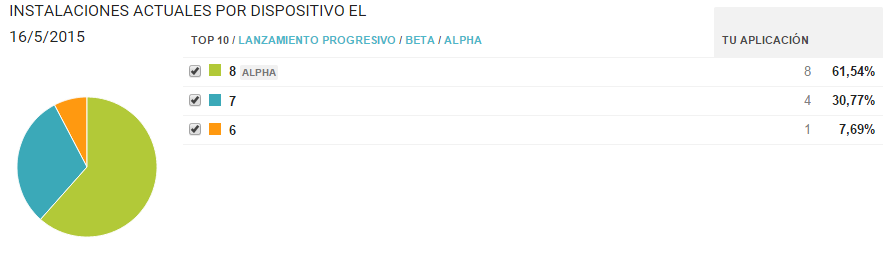
\includegraphics{figs/InstalacionesActuales.png}} 
    \caption{Instalaciones actuales de Baldugenda Console Developer} 
    \label{fig:InstalacionesActuales} 
  \end{center} 
\end{figure}

Las opciones de gráficos facilitan saber cuántos usuarios han actualizado a la versión nueva y cuántos se mantienen en versiones anteriores.
También da la posibilidad de verlo mediante una escala de tiempo


\begin{figure}[H] 
  \begin{center} 
    \scalebox{1}{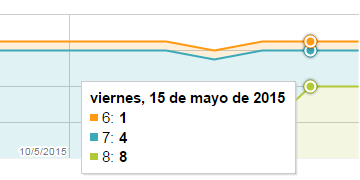
\includegraphics{figs/EscalaTiempo.png}} 
    \caption{Escala de tiempo Console Developer} 
    \label{fig:EscalaTiempo} 
  \end{center} 
\end{figure}

Aparte de todo esto, Google promociona el uso de Google analytics, un servicio web para recopilar datos de interacción del usuario en las aplicaciones que se generen.
En la aplicación de Baldugenda se decidió usar una API de terceros llamada Splunk Mint que se detallara mas adelante para la labor de recopilar información sobre los fallos en la aplicación.
 Al realizar acciones de debugging hay que ponerse en todas las situaciones posibles en las que se pueda llegar a estar en la aplicación, al ser una aplicación móvil no siempre se tendrá la misma cobertura de Internet o las cuentas de Google podrán modificarse.

También puede darse el caso que el móvil falle y se tenga que borrar,  todas estas situaciones hay que tenerlas en cuenta, una de las situaciones que no se suele tener presente cuando no se esta acostumbrado a realizar aplicaciones para móviles es que hay dos posiciones y que dependiendo de que posición se tenga el móvil puede que la información se vea distinta o directamente no se vea.
Puede darse el caso que falle la aplicación en algún punto crítico como puede ser la realización de una escritura en la base de datos o en una llamada al servidor, esas situaciones suelen ser muy comunes al no estar conectado a Internet  todo el rato.

Como al principio no se puede pretender que se sepa en donde va a fallar en cada momento, viene bien instalarse la opción que da Google con su Google analytics o otras opciones de terceros como Splunk mint.
Ya que mientras los usuarios que están haciendo pruebas les falla, se puede configurar para que te llegue al correo el motivo por el que la aplicación ha dejado de funcionar y en que  lineas se ha producido el fallo, gracias a esta información ya se pueden sacar conclusiones de porque ha fallado y como se podría solucionar. Vale de poco pasarse horas y horas probando casos que igual se producen 1 de cada 100.000 veces cuando se ha podido pasar un caso que a una tercera parte de los usuarios les va a suceder.

Los usuarios, la mayoría no sabrán decir lo que les ha pasado cuando ha fallado la aplicación ni tan siquiera lo que estaban haciendo cuando ha dejado de funcionar, por este motivo tener a un chivato que nos diga al menos que botón han pulsado es útil.
 


\subsection{Notificaciones}
\label{subsecc:Notificaciones}

Google proporciona un servicio de notificaciones push muy potente llamado Google Cloud Messaging (GCM), este servicio permite hacer que aparezcan esos mensajes en la pantalla de arriba del móvil cuando llega un mensaje o cuando nos piden vidas en los juegos de las redes sociales.
Gracias a estas notificaciones no se necesita tener la aplicación conectada ya que trabajan sobre un servidor y es el servidor quien se pone en contacto con nosotros.

En el caso de Baldugenda no se han usado este tipo de notificaciones, el uso de notificaciones se ha limitado a las que vienen con los eventos que genera Google Calendar.
Al crear un evento, si el calendario tiene la opción de realizar notificaciones cuando se vaya a producir el evento,   el evento se creara sin ninguna alarma programada pero el propio calendario avisara al usuario con una notificación al móvil o a la versión web si tiene la versión web de Google Calendar abierta.
Para que se produzca la notificación en el móvil el calendario tiene que estar sincronizado con el móvil y actualizado para que se haya cargado los eventos nuevos desde la ultima sincronización, si no se da esa situación la notificación no saltara.
Se decidió no meter alarmas en los exámenes porque eso obligaría al usuario a tener que estar metiéndose en la aplicación cada vez que quisiera desactivar la alarma en cambio al realizarlo mediante Google Calendar y la creacion de eventos, el usuario es libre de realizar las modificaciones en Google Calendar y tener los exámenes en un calendario con las notificaciones activadas.

\subsection{Backup}
\label{subsecc:Backup}

La necesidad del Backup es algo importante en cualquier aplicación en la que el usuario tiene que meter algún dato, a nadie le gusta perder información que ha estado gastando su tiempo escribiendo. Los móviles suelen romperse o estropearse y en esas situaciones perder todo supondría un grave problema, para esas situaciones una copia de seguridad es el mejor salvavidas.
Para el Backup Google tiene opciones tales como las propias implementadas en Android el backup API, que aunque hemos separado las explicaciones en Google y Android, Google compró Android en 2005 y muchas funcionalidades que se pueden encontrar en Android están vinculadas con Google.

Tambien tiene otras opciones más simples como puede ser usar una opción de respaldo en la nube de Google Drive\cite{GDrive}, transparente para el usuario.
La primera opción la ventaja que tiene es que el usuario no tiene que realizar ningún paso para realizar la copia de seguridad, es el propio desarrollador quien prepara todo, pone la clave de la aplicación que se usa en todas los servicios Google para vincular la aplicación con el servicio y después el sistema realiza el backup donde el desarrollador lo escoja. Y Google guarda la información en la nube sin que el usuario pueda acceder a ella, solo se podrá acceder a esa información por medio de la aplicación que ha realizado el backup.

\begin{figure}[H] 
  \begin{center} 
    \scalebox{1}{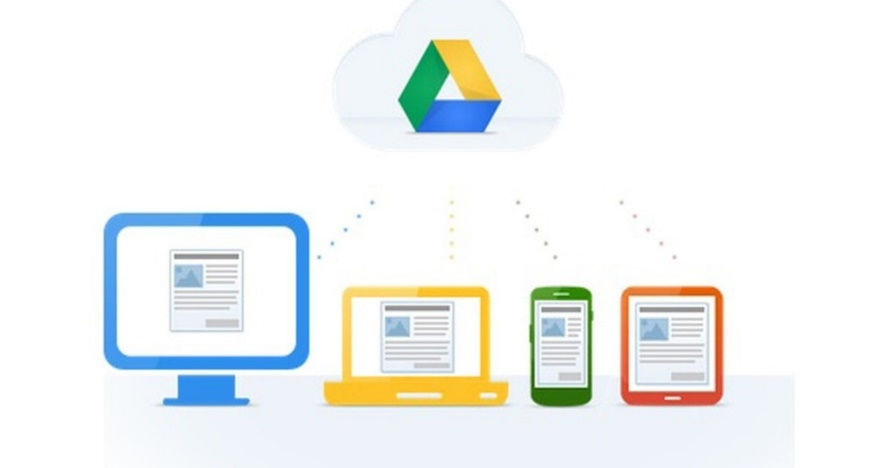
\includegraphics{figs/Drive.png}} 
    \caption{Google Drive Google} 
    \label{fig:Drive} 
  \end{center} 
\end{figure}

La segunda opción parece que tiene más problemas que ventajas pero dependiendo de cómo se use puede ser incluso más útil que la primera.
En esta segunda opción el usuario puede ver en todo momento donde está su información alojada y si no se fía de tenerla en Google Drive puede descargarla y guardarla en su ordenador o mandarla por email.
El problema de tener la copia de seguridad tan accesible es que el usuario puede modificar el fichero, esto podría ser un problema pero con una buena seguridad a la hora de importar la base de datos, esas situaciones no tendrían que repercutir en la aplicación.
Al estar implementando la parte de backup en Drive se encontró que por cada aplicación que se instala los desarrolladores pueden usar una parte del Google Drive si se les da permiso que ni los propios usuarios podrán tocar y sirve como carpeta de preferencias la cual al borrar la aplicación desaparecería.

En Baldugenda esa carpeta no se usó ya que ya se había empezado a usar el sharedpreferences de Android, pero si en alguna aplicación futura se quisiera reducir el espacio que ocupa la aplicación esta carpeta podría resultar de utilidad.
Otra de las ventajas de realizar la copia en Google Drive es que si en un futuro se quisiera compartir información entre usuarios de Baldugenda solo se tendría que modificar la opción de importar y agregar una opción de juntar agenda existente. Con esto se podrían compartir exámenes, asignaturas y el usuario no tendría que estar metiendo las asignaturas ni los exámenes.

El uso de Google Drive es sencillo ya que tiene 3 formas de usarlo y ofrece documentacion para cada una de las formas, mediante REST, mediante la librería java o mediante el sdk de Drive.
El ejemplo que ofrece Google es con el sdk de Drive así que Baldugenda tiene implementada esta opción en el código de Github.
Google Drive ofrece muchas posibilidades a la hora de crear las carpetas y subir los ficheros, se pueden crear ficheros usando tus propias actividades en Android y rellenando todo o puedes usar una actividad que proporciona Google Drive para crear y seleccionar ficheros.

Para el usuario es mucho más cómodo mostrarle algo que le resulte familiar a la hora de hacer elecciones y por eso se optó por usar las actividades que proporciona Google Drive aparte de que tiene un diseño refinado y una cantidad de opciones y posibilidades asombrosas.
Se dieron ciertos problemas a la hora de realizar el backup con Google, ya que al crear carpetas en Drive o ficheros, no se producen inmediatamente y hay situaciones en los que por diversos motivos el servidor está ocupado y tarda un poco más, en esas situaciones el identificador de la carpeta no era accesible desde el momento que se generaba y tardaba un tiempo, esto hacía que fallara seleccionar la carpeta donde el sistema subiria el fichero.
Por ese motivo se decidió separar la parte de la selección de la carpeta de la parte de exportación de la BD.

\subsection{Problemas al desarrollar con Google}
\label{subsecc:Problemas al desarrollar con Google}

La mayoría de los problemas que se encuentran cuando se está trabajando con Google es por el uso de los servicios de Google dentro de la aplicación.
Cuando se intenta implementar algún servicio de Google hay que leerse muy bien el manual del servicio y comprobar que este actualizado. Google tiene un poco desordenado su documentación de los servicios, la ha separado tanto y con tantos enlaces que a veces llega a ser confuso.
Al principio Google explica dentro de su web de APIs que utilidades tienen y como sacarles partido. Para ello separa cada API y hace una especie de guía y después pone un apartado para que se empiece a programar y aquí es donde empieza la confusión, Google suele añadir enlaces a muchos sitios dentro de su documentación para explicar lo más básico del manual, por este motivo hay que tener muy claro donde se tiene que buscar la información.

Una manera de hacer frente a este problema es buscar tutoriales por Internet o video tutoriales donde implementen ese API, y de ahí ya seguir con las funciones propias que tendrá tu aplicación.
El apartado de los credenciales es igual el punto que mayores problemas causan a la hora de hacer que funcione una API al principio, dependiendo qué modo se use, se tiene que activar unas credenciales u otras, aparte cada API necesita un tipo de credencial distinta dependiendo a que recursos quiera acceder la aplicación.
Por ese motivo lo mejor es familiarizarse con la API fuera del proyecto, creando un proyecto pequeño y haciendo que funcione la API por separado y después incluirlo ya funcionando al proyecto que se quiere implementar.
Google dispone de ejemplos en Github de sus APIs, el problema es que esos ejemplos no suelen estar actualizados o no están en todos los modos en los que Google lo ofrece, por ejemplo el API de Google Calendar que se usó en Baldugenda.Google ofrece un acceso a esa API por medio de REST, al ir a buscar ejemplos para esa API se dieron casos de todo tipo, al ser un API que ya tiene distintas versiones, había ejemplos de cada una de ellas pero  de API REST para Android pocos o que no explicaban bien el código. Y en el Github de Google el único ejemplo que había para el API de Google Calendar era haciendo uso de la librería en java.

Aparte del uso de las APIs en Google, otros problemas que han surgido han sido al compartir el enlace de descarga de la aplicación.
La primera opción para compartirlo fue por medio de una comunidad de Google plus,  el fallo que se encontró fue que había algunos Baldusers que no tenían cuenta en Google plus y no querían creársela, así que no podían acceder a la descarga de la aplicación.
Para esos casos se usó los grupos de Google para invitarlos a esos grupos y que pudieran descargarse la aplicación desde ahí.
Algunos Baldusers experimentaron problemas al actualizar baldugenda ya que hay un error en Google play ya reportado por los comunidad de desarrolladores de Google que sucede al corromperse la información de las cuentas vinculadas al dispositivo móvil, por ese motivo Google no permite descargar aplicaciones y exige mucho más espacio del requerido.

Para solucionar el problema se estuvo investigando y la solución era quitar la cuenta de Google del dispositivo y volverla a poner desde cero.
Con eso el Google play cargaría de nuevo la lista de aplicaciones y sus actualizaciones y funcionaria la descarga.
El problema ocasionaba que se les exigía un espacio de memoria altísimo para 2 Mbs que pesaba la aplicación y al no tener espacio suficiente les daba un error al actualizar.


\begin{figure}[H] 
  \begin{center} 
    \scalebox{1}{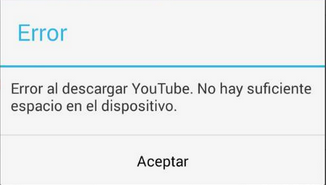
\includegraphics{figs/ErrorGoogle.png}} 
    \caption{Error Google Play} 
    \label{fig:ErrorGoogle} 
  \end{center} 
\end{figure}

Ahora se hablara de problemas más específicos con respecto al calendario y al Drive.

\subsubsection{Problemas Google Calendar}
\label{subsubsecc:Problemas Google Calendar}

Un problema que no se pudo solucionar mediante código fue el problema de la sincronización de Google Calendar con el dispositivo móvil. La idea principal era que cuando se realizaban nuevos eventos en el calendario estos eventos se sincronizaran automaticamente con el calendario del dispositivo, si el Balduser no tenía activada la sincronización por tiempo y la tenía manual no le aparecería en su móvil a menos que le diera a sincronizar.
Para solucionarlo se les comunicó como hacerlo a los Baldusers y los que lo vieron necesario lo usaron.
Otro problema que se encontró al implementar las opciones de calendario fue el uso de la autenticación OAuth2 \cite{Oauth} que requiere el API.
Las explicaciones eran muy confusas a la hora de configurar ya que las ventanas y las opciones que aparecían en la guía de Google eran de versiones anteriores a las configuraciones que tenía que realizar yo.
La forma de solucionarlo fue viendo vídeos donde otros desarrolladores creaban credenciales para APIs de Google que requirieran ese tipo de credenciales y haciendo pruebas se consiguió que empezara a subir la cuota de uso.


\subsubsection{Problemas Google Drive}
\label{subsubsecc:Problemas Google Drive}

Google Drive no dio tantos problemas como en su momento Google Calendar, aun y todo se tuvieron algunos problemas a la hora de implementar la API.
Para facilitar el trabajo con Google Drive y habiendo aprendido de Google Calendar se decidió no perder el tiempo buscando como crear las funciones desde cero y se optó por descargar el ejemplo y coger lo necesario y adaptarlo a Baldugenda.
Cuando se importó el proyecto todo era muy confuso y no se parecía a la forma de trabajar que se había seguido anteriormente en Google Calendar.
Aun y todo se miró el código, se entendió más o menos lo que hacía en cada función,  y se intentó sacar las funciones necesarias al caso de uso de Backup de Baldugenda.
Cuando se sacaron las funciones y se comprobó que funcionaba la selección de ficheros por un lado y la subida de ficheros por otro se intentó juntar.

El problema fue que Google al crear una carpeta mediante el \gls{activity} que dan de ejemplo pasa un tiempo hasta poder usar el identificador de esa carpeta. Y eso producía un fallo en el código ya que al intentar subir a una carpeta que no tenía identificador fallaba el programa.
La solución fue separar por una parte la selección de la carpeta y por otra la subida del fichero, con eso se le daba tiempo a Google a que generara el identificador y de paso el usuario podía comprobar que la carpeta se había seleccionado correctamente.
Antes de optar por esa solución se pensó usar las preferencias de la aplicación para guardar la dirección donde se guardaba la carpeta y de esa manera poder realizar backups periódicos sin depender del usuario, pero el problema seguía siendo el mismo así que se descartó esa opción.

Cuando se implementó el backup no se tuvo en consideración el uso distintos usuarios de Google en el mismo dispositivo. Así que al hacer las pruebas todo iba bien ya que no se modificaba la cuenta, en cambio al usuario sí que se le daba la posibilidad de cambiar las cuentas del Calendar para guardar las cosas. Al ser la forma de conexión distinta no se consiguió usar los certificados creados para el Calendar dentro del Drive.
Se investigó por Internet y en StackOverflow un usuario dio la solución que era agregando el API de Google plus, realizando un borrado del cache de los credenciales y desconectando y volviendo a conectar, ya pedía de nuevo el email de la cuenta a la que se quería acceder.

\newpage
Si se quiere desarrollar una aplicación en Android este es una de los puntos más importantes de esta memoria ya que se detallara los puntos más importantes y los problemas que se han tenido al desarrollar la aplicación y problemas que pueden surgir.
Para empezar, lo más importante ¿Por qué programar en Android y no en otro SO?
El motivo por el que Baldugenda está para Android  y no es multiplataforma es que se quería 
comprobar el potencial que tiene Android y centrarse en esta plataforma.
Aparte si hablamos de números podemos ver cómo están actualmente los sistemas operativos en el mercado móvil.

\begin{figure}[H] 
  \begin{center} 
    \scalebox{0.6}{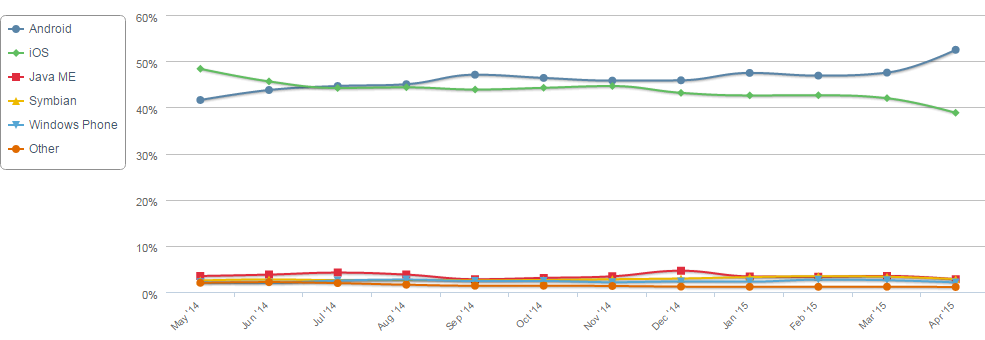
\includegraphics{figs/TendenciasSO.png}} 
    \caption{Tendencias en móviles SO netmarketshare.com} 
    \label{fig:TendenciasSO} 
  \end{center} 
\end{figure}

Se puede ver que a principios de este año Android le ha cogido la delantera a iOS, los dos son líderes en el mercado móvil.
Google ha conseguido resolver la fragmentación de sus versiones de Android y eso le ha dado dolores de cabeza a iOS la cual ha pasado a ocupar el segundo lugar.
\newpage
\begin{figure}[H] 
  \begin{center} 
    \scalebox{1}{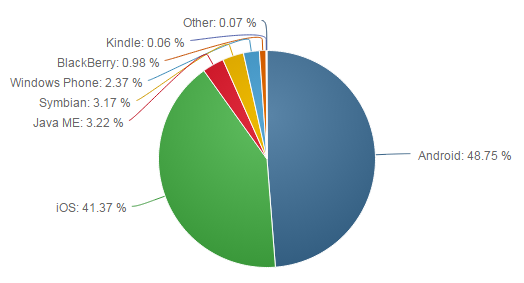
\includegraphics{figs/RankingSO.png}} 
    \caption{Ranking de móviles SO netmarketshare.com} 
    \label{fig:RankingSO} 
  \end{center} 
\end{figure}

El motivo anterior sumado al aumento de personas que usan Android en sus dispositivos y siendo un usuario de Android en estos momentos, me llevó a la decisión de querer sacarle el máximo partido realizando una aplicación nativa en Android.
Antes de comenzar a desarrollar en Android hay ciertos aspectos que hay que saber.
Uno muy importante es que se necesita conocimientos de Java.
Y estar acostumbrado a trabajar con programación orientada a objetos.
Aparte de estos dos anteriores, un IDE que actualmente el que más auge tiene entre los desarrolladores de Android es el Android Studio por su facilidad a la hora de crear un proyecto.
Y muchas ganas de aprender.
Si se tiene todo lo anterior programar en Android no resultará complicado. Al principio parecerá todo un poco lioso pero el periodo de aprendizaje después compensa ya que lo que al principio tardarías en hacerlo 3 horas al cabo de 2 semanas podrás hacerlo en 10 minutos porque ya te sabrás la mayoría de funciones principales en Android.


\subsection{Restricciones de API}
\label{subsecc:Restricciones de API}

Ya se ha comentado anteriormente que Google ha ganado terreno en el mercado de los móviles por su labor en la desfragmentación de Android, aun con la labor de Google los desarrolladores nos seguimos encontrando que si no cogemos las versiones antiguas de Android y solo desarrollamos para las nuevas quitaremos una parte importante de los usuarios.

\begin{figure}[H] 
  \begin{center} 
    \scalebox{1}{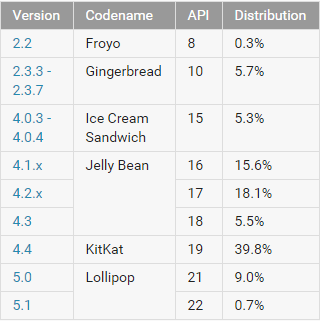
\includegraphics{figs/VersionesAndroid2.png}} 
    \caption{Versiones Android developer.android.com} 
    \label{fig:VersionesAndroid2} 
  \end{center} 
\end{figure}

Estas estadísticas son de mayo de 2015, si se quiere conservar a la mayor cantidad de gente y no limitarse mucho con la aplicación los expertos recomienda empezar a olvidar a la gente que tiene GingerBread para abajo.
En la aplicación de Baldugenda se cogió también a los de API 10 ya que las funciones que se iban a implementar no suponían gran avance tecnológico en cuanto a versión de Android así que se podía usar perfectamente la versión 10 sin verse limitado.
Al coger API más bajas uno se expone a tener que realizar más código especial para esas versiones antiguas e invertir tiempo en retocar cosas para que no se note la diferencia y que el usuario no tenga problemas de interacción.

 
Cada una de las APIs mostradas arriba añade diferentes funciones, la más destacada la se puede ver comparando el API 10 con el API 21, el apartado grafico que usa Android en una u otra varía mucho dependiendo de la versión que se use como mínimo.
Más adelante se explicara la interfaz en Android, pero para ver la diferencia y el coste que aumentaría usar una API de más bajo nivel del necesario, se puede ver en la barra de arriba de los dispositivos móviles. A partir del API 21 Android ha optado por un diseño llamado Material Design, este diseño produce que el usuario vea la aplicación más cercana al trabajar con sombras, distintas profundidades y colores más llamativos.
El problema surge cuando se quiere usar este diseño en APIs más bajas, Google proporciona documentación para realizar el material design sobre versiones anteriores a Lollipop, pero aun y todo con toda esa información la diferencia entre usar un API como la 21 frente a usar un API 10 cambia mucho.


\begin{figure}[H] 
  \begin{center} 
    \scalebox{1.2}{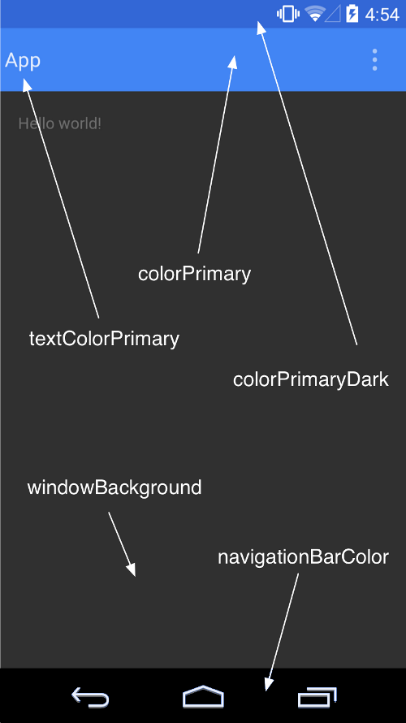
\includegraphics{figs/AndroidToolbar.png}} 
    \caption{Android Toolbar colores android-developers} 
    \label{fig:AndroidToolbar} 
  \end{center} 
\end{figure}

En la imagen mostrada arriba se puede apreciar cómo funcionan los colores en Android desde la versión 21, en cambio si se quiere conseguir algo parecido a eso hay que implementar clases que hagan lo mismo, y no se puede basar solo en las librerías de compatibilidad que ofrece Google.
Un componente que agregó el API 21 fue la toolbar que como se pude ver también permite cambiar el color de la barra donde se encuentra la hora, etc…
En el API 10 el resultado final es muy parecido pero se invierte bastante tiempo, que si el diseño no es primordial, molesta gastarlo agregando colores.

\subsection{Tipo de dispositivos}
\label{subsecc:Tipo de dispositivos}

Android a diferencia de IOS tiene una gama demasiado grande de dispositivos, muchas empresas usan el sistema operativo de Android para sus móviles.
Por este motivo cuando se quiere desarrollar para Android hay que saber muy bien a que dispositivos se quiere dirigir la aplicación.
Los dispositivos Android pasan desde una pantalla de televisión, hasta un pequeño smartwatch.
Hay que saber que dispositivos quitar para llegar a la mayor parte de los usuarios que se quiere que usen la aplicación.
Para resolver la duda Google ofrece periódicamente las estadísticas de los dispositivos usados y sus versiones.
De las versiones ya se ha hablado en un tema anterior, ahora en este apartado se hablara de las densidades y los tipos de pantalla.

\begin{figure}[H] 
  \begin{center} 
    \scalebox{0.7}{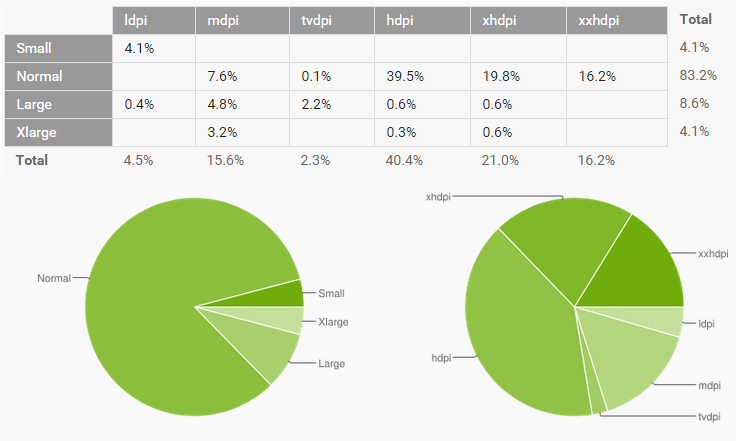
\includegraphics{figs/ComparativaPantallas.png}} 
    \caption{Comparativa tipo de pantallas developer.android.com} 
    \label{fig:ComparativaPantallas} 
  \end{center} 
\end{figure}

Estos datos los proporciona Google, actualizado en mayo de 2015.
Se puede apreciar las distintas gamas que hay de dispositivos. A la hora de crear el proyecto si se usa Android Studio,el IDE dara consejos con estos temas preguntándote hacia que dispositivo va destinada la aplicación y se tendra  que elegir entre móviles o tablets, televisión, aparatos wear de Android, o las Google glass.
Dependiendo de que elección se escoja en ese momento se modificaran automáticamente los ajustes para que el proyecto esté preparado para el dispositivo seleccionado.
Baldugenda es una aplicación destinada a móviles y tablets ya que su uso está pensado para ser algo habitual y de acceso rápido.
Las aplicaciones que se desarrollan del estilo de Baldugenda suelen ser para móviles también ya que tienen que hacer la función de agenda virtual. Eso no quita para que también haya widgets de esas aplicaciones compatibles con dispositivos como los smartwatch donde se reciben las notificaciones de las aplicaciones de este género.

\subsection{Interfaz}
\label{subsecc:Interfaz}

Uno de los problemas más grandes que se encuentra uno al desarrollar en Android y en cualquier sistema operativo para dispositivos móviles es la limitación de espacio en la pantalla de aparato, también al haber distintos tipos de pantallas hacerlo compatible con todos es una tarea ardua.
Hay muchos aspectos que hacen que los usuarios no borren la aplicación, como puede ser que les parezca entretenida o útil, pero por mucho que una aplicación cumpla todo eso por debajo, a los usuarios se les gana por la vista. Si se quiere mantener la aplicación instalada en los dispositivos de los usuarios tiene que ser agradable para la vista y también cómoda de usar.
De algo que la mayoría de los informáticos pecamos es que el diseño no es un aspecto importante dentro de nuestra labor y por muy divertida que hagamos la parte lógica de la aplicación después el diseño se resiste a salir bien.

Pero aun y todo evitando este tema hay que dedicarle un tiempo después de haber finalizado la parte lógica y antes de publicar la aplicación al apartado de diseño.
Unos colores vivos frente a un fondo blanco marcan la diferencia.
En el caso de Baldugenda durante la primera fase se decidió hacer los casos de uso y que fueran los Baldusers los que dieran propuestas de diseño que les parecieran más atractivas.
De esa forma se pasó de un menú principal de 6 botones grises y un fondo blanco a 6 iconos con fondo de colores.

Android proporciona muchos componentes para retocar la interfaz a la hora de desarrollar algunos tan vistosos como un ExpandableList y otros que pasan desapercibidos como puede ser un TextView.
Lo más importante es sacarle provecho a la pequeña pantalla sobre la que se está trabajando y usar dispositivos con pantalla pequeña para realizar las pruebas. Ya que estos casos son los más peligrosos, en el caso de que sobre mucho espacio en un dispositivo de tamaño más grande siempre se podrá meter algo más dependiendo del tamaño pero si el dispositivo tiene la pantalla demasiado pequeña hay que saber comunicar al usuario para que no se pierda en la aplicación.

 
Algo muy vistoso y que no debe faltar en ninguna aplicación son los menús laterales, estos menús no ocupan espacio para el usuario y cuando él quiere los abre y los cierra.
\newpage
\begin{figure}[H] 
  \begin{center} 
    \scalebox{0.7}{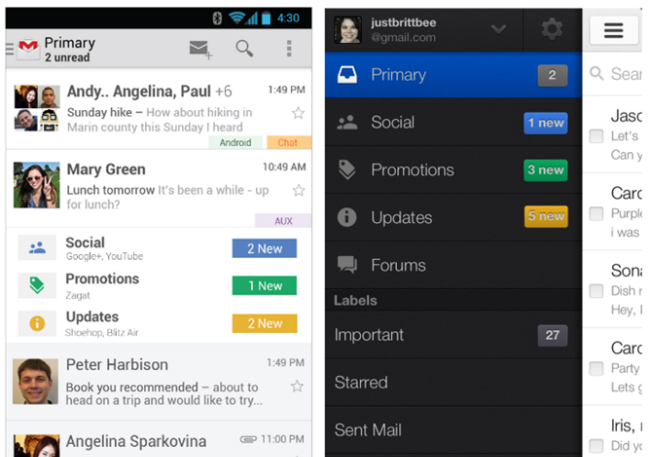
\includegraphics{figs/MenuLateral.png}} 
    \caption{Menu lateral Gmail} 
    \label{fig:MenuLateral} 
  \end{center} 
\end{figure}

En Baldugenda se puso un menú de este tipo en la lista de exámenes y les pareció interesante a los usuarios.
Algo que como desarrolladores hay que aprender es que la aplicación si se quiere publicar para que sea descargada por todo el mundo tiene que tener funcionalidades que a los usuarios les parezcan interesantes y por ello deben ser los propios usuarios los que den ideas de nuevas funcionalidades para futuras mejoras. La aplicación tiene que ir destinada a los usuarios y por este motivo ellos no se van a fijar en la dificultad que tiene sacar la información de la base de datos y mostrarle justo lo que buscan cuando lo buscan.
A ellos lo que les importa principalmente es que sea impactante y divertida a la hora de interactuar con ella.
Si se cambia un botón por algo distinto donde el usuario arrastre o realice otra acción eso le sorprenderá.

El ejemplo que se encontró en Baldugenda es al realizar borrados y modificaciones.
Dependiendo del usuario que la ejecutaba y la edad que tuviera estaban más acostumbrados a las acciones especiales de los botones como mantener pulsado o arrastrar.
Un punto interesante también son los Dialogs, ventanas que se muestran superpuestas a la actividad que se está ejecutando. Gracias a esos dialogs se gana mucho espacio y se consigue que el usuario preste atención a la zona donde se quiere en cada momento.

Volviendo a las pulsaciones largas y juntándolo con el tema de los dialogs en Baldugenda se juntó todo esto y usaron los menús para realizar acciones sobre un objeto en específico.
Los expandable list view es una buena forma de mostrar listas muy largas de lo que se precise agrupándolas por un motivo en concreto.
De esta forma el usuario no tendrá una lista que le ocupa la pantalla, en vez de eso tendrá cajitas, que abriendo una tendrá lo que busca de esa categoría.


\begin{figure}[H] 
  \begin{center} 
    \scalebox{0.7}{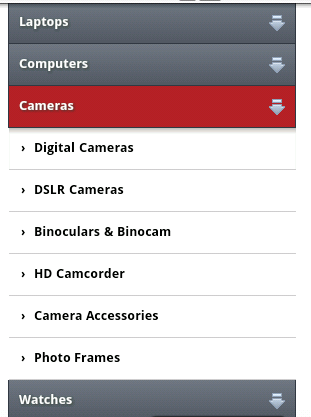
\includegraphics{figs/ExpandableList.png}} 
    \caption{Expandable list view} 
    \label{fig:ExpandableList} 
  \end{center} 
\end{figure}

En este punto también entra el toque artístico de cada persona, cada caja se puede diseñar de la forma que el desarrollador quiera y también añadir los colores.

\subsection{Migración}
\label{subsecc:Migración}

Cuando se decidió implementar en Android se descartó usar aplicaciones para desarrollar multiplataforma.
Por este motivo hubo que mirar las posibilidades que había y las dificultades que se encontraría si se tuviera que implementar Baldugenda por ejemplo para IOS o Windows Phone.
Microsoft se ha adelantado a la compañía del Androide y de la manzana y ha optado por ayudar a los desarrolladores a migrar aplicaciones desde IOS y Android a Windows Phone.
Esta medida se debe a las estadísticas que se han podido ver sobre los smartphones y el tipo de sistema operativo que usan.

Para ello ha ideado una API estilo diccionario para ver las equivalencias entre Android y Windows phone y con eso hacer más fácil a los desarrolladores la conversión de las clases y las funciones.
Entre IOS y Android no es tan fácil la migracion. Los dos son empresas muy fuertes en el mercado de los móviles y no darían su brazo a torcer para ayudar a su competidora.
Pero algo positivo que tiene trabajar con un modelo MVC es que cada apartado está separado.
El modelo se podría trasladar directamente a IOS y la parte de la vista y controlador se podría distribuir entre más personas para desarrollar sobre el ejemplo de Android.
Cuando se habla de migraciones siempre se viene a la cabeza cambio de sistema operativo y cosas así, pero también una migración podría ser el salto de una aplicación móvil a un dispositivo wear de Android o a una pantalla de televisión. Para eso el cambio vendría a ser muy parecido pero pudiendo usar gran parte del código exceptuando cosas como la parte de la vista y la conexión entre la vista y la lógica.

Un punto importante que hay que tener en cuenta a la hora de migrar no es solo instalar la aplicación en un nuevo dispositivo, hay que pensar en los usuarios y permitirles llevarse todo lo realizado hasta el momento en la aplicación anterior a la nueva.
Hay aplicaciones que guardan la información en sus propios servidores y ese paso es transparente para el usuario.
En cambio en el caso de Baldugenda al no usar ningún servidor exceptuando el de Google Calendar para guardar los exámenes, se decidió poder migrar los datos mediante la opción de exportar base de datos y usar la cuenta de Google para pasar de un dispositivo a otro.

\subsection{Notificaciones}
\label{subsecc:Notificaciones}

Las notificaciones en Android es un componente importante dentro de las aplicaciones. Es la forma con la que la aplicación se comunica con el usuario.
Hay distintos tipos de notificaciones:
Están las notificaciones Toast que son mensajes que se escribirán en la pantalla durante un periodo largo o corto según se le indique.
\newpage
\begin{figure}[H] 
  \begin{center} 
    \scalebox{0.7}{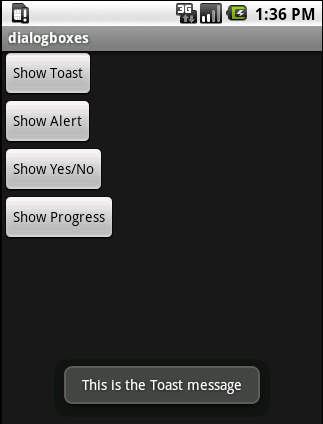
\includegraphics{figs/NotificacionToast.png}} 
    \caption{Notificación Toast} 
    \label{fig:NotificacionToast} 
  \end{center} 
\end{figure}

A la hora de realizar la aplicación si no se encuentra dónde está el fallo, una forma muy útil de usar las notificaciones Toast es sacar por este mensaje los valores que nos interesen para saber si se está trabajando sobre el objeto que se necesita.
Dentro de Baldugenda se ha usado los Toast para comunicar al usuario que se había creado un examen o una asignatura. Hay veces que el teclado tapa estos mensajes así que hay que tener cuidado en qué momento se escriben porque puede que el usuario no lo vea.

Otro tipo de notificaciones son los alertdialog y los timepicker dialog y datepicker dialog.
El alertdialog admite un título, un texto y como máximo 3 botones. Se suele usar para hacer que el usuario confirme una acción, en Baldugenda se ha usado a la hora de borrar la asignatura se le pregunta sí está seguro de borrarla, si pulsa que si la asignatura se borrara en cambio sí cancela no habrá pasado nada.
\newpage
\begin{figure}[H] 
  \begin{center} 
    \scalebox{0.7}{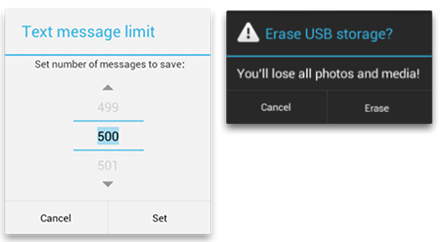
\includegraphics{figs/EjemplosDialog.png}} 
    \caption{Ejemplos de dialog} 
    \label{fig:EjemplosDialog} 
  \end{center} 
\end{figure}

Tanto el timepicker dialog como el datepicker dialog son ventanas modales que actúan sobre la hora y la fecha respectivamente.
Se le da la opción al usuario que escoja el dia mediante el datepicker y mediante el timepicker puede seleccionar la hora.

Dependiendo de la versión del dispositivo estas ventanas modales serán de una forma u otra.

\begin{figure}[H]
 \centering
  \subfloat[Ejemplo DatePicker en Lollipop]{
   \label{f:Ejemplo DatePicker en Lollipop}
    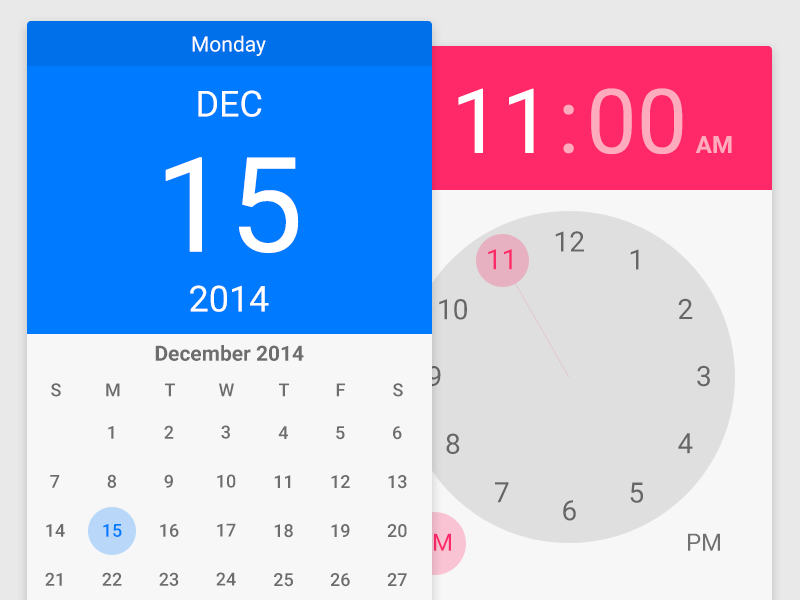
\includegraphics[width=0.4\textwidth]{figs/DatePickerLollipop.png}}
  \subfloat[Ejemplo DatePicker en JellyBean]{
   \label{f:Ejemplo DatePicker en JellyBean}
    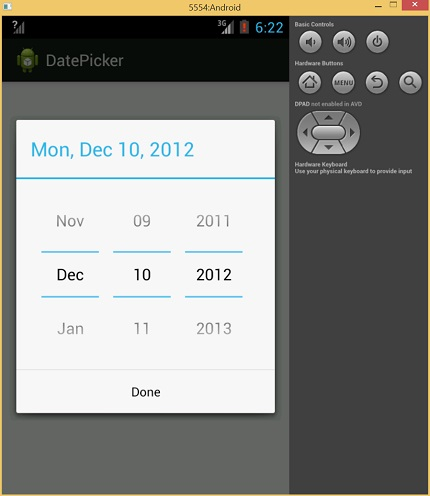
\includegraphics[width=0.4\textwidth]{figs/DatePickerJellyBean.png}}
 \caption{Tipos de DatePicker dependiendo de la version}
 \label{f:Tipos de DatePicker dependiendo de la version}
\end{figure}

A la izquierda podemos ver el datepicker en la versión de lollipop y a la derecha un una versión anterior.
Para el manejo de los días se usa la clase Calendar de java y eso ha venido muy bien ya que Google Calendar sus funciones permiten directamente meter una fecha creada en un objeto Calendar al evento.
De esa forma el trabajo que hubiera supuesto tener que sacar la fecha actual calcular cuánto falta hasta la fecha elegida por el usuario y demás, se quita y solo se tuvo que sacar la información que seleccionaba el usuario e insertarla en el evento.

Aparte de estas notificaciones tenemos  una muy importante si se va trabajar con servicios de Google que es el progress dialog.
Este tipo de componente es muy útil con estos servicios ya que al usar los servicios de Google hay veces que las conexiones tienen que hacerse en segundo plano y hay que lanzar tareas asíncronas, pero se sigue dependiendo del resultado del servicio para seguir trabajando.
Con este componente se genera una barra de progreso que se irá llenando según avance la tarea asíncrona o directamente un mensaje que no dejará realizar ninguna otra acción hasta la finalización de la tarea asíncrona.
En Baldugenda se le ha dado uso al realizar la búsqueda de los calendarios y al realizar la creación de exámenes, porque dependiendo de la velocidad que tenga el móvil por Internet, puede que el servicio de Google Calendar no vaya lo más rápido que debería y dé error si dejamos que se genere en la ventana secundaria sin avisar al usuario. 

\begin{figure}[H] 
  \begin{center} 
    \scalebox{0.8}{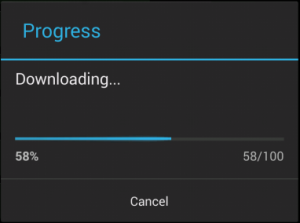
\includegraphics{figs/ProgressDialog.png}} 
    \caption{Ejemplos de ProgressDialog} 
    \label{fig:ProgressDialog} 
  \end{center} 
\end{figure}

Mostrarle al usuario una ventana explicándole lo que está pasando en cada momento hace que no se ponga a pulsar todos los botones pensando que se le ha quedado parada la aplicación.
Se han dado situaciones en el proyecto que por no avisar al usuario que se había generado un examen mediante una ventana de progress dialog, el usuario se pensaba que no estaba generada y la intentaba crear otra vez con el consiguiente error.
Por eso es una buena opción si se quiere llamar la atención del usuario, si lo comparamos con los toast esta opción es más engorrosa pero el usuario la vera aunque tenga el teclado abierto.

\subsection{Uso de calendarios}
\label{subsecc:Uso de calendarios}

Ya se ha hablado de los timepicker dialog y datepicker dialog en el apartado de las notificaciones de Android.
En este punto se hablará más a fondo del uso que se le suelen dar a los calendarios en las aplicaciones del tipo Baldugenda.
Android tiene un calendario dentro del dispositivo que si no se le asocia ninguna cuenta trabajará con eventos en local. Muchas aplicaciones usan este calendario para generar ahí los eventos, otras simplemente crean su propio calendario dentro de la aplicación.
El problema que se vio al generar el calendario dentro de la aplicación era que el usuario tenía que estar duplicando los eventos si quería tenerlo siempre disponibles.
Una de las mejoras que se tiene pendiente en Baldugenda es la visualización de los eventos en formato mes.

\begin{figure}[H] 
  \begin{center} 
    \scalebox{0.8}{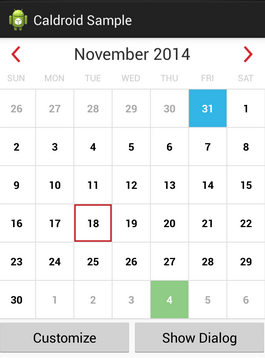
\includegraphics{figs/Caldroid.png}} 
    \caption{Ejemplo de Caldroid Github} 
    \label{fig:Caldroid} 
  \end{center} 
\end{figure}

Como se puede observar en la imagen esa sería un tipo de ventana que se quiere implementar en la aplicación Baldugenda para mostrar por días los exámenes que se tienen apuntados.

Por falta de tiempo no se realizó, aunque sí se tenían propuestas librerías para realizar este tipo de vista como puede ser caldroid una librería con copyright disponible en Github que ofrece las funciones necesarias y el diseño, para mostrar el calendario de esta forma y poder generar eventos y marcarlos de colores.
Aun y todo se seguiría usando Google Calendar para mantener consistencia a los calendarios del usuario y que tenga acceso siempre a los eventos que se generan dentro del móvil.
Android ofrece su propio componente de vista de calendario, el Calendar view, el problema que se encontró al usarlo es las limitaciones visuales que tiene, se buscaba al usar ese vista mostrar los exámenes que había en el mes, y con Calendar view no se podía agregar eventos a los días del calendario.

Por ese motivo se decidió dejar el tema de la vista del calendario como algo secundario y centrarse en cosas más importantes como el backup
Se ha probado a instalar muchas aplicaciones que tienen la finalidad de guardar asignaturas y exámenes en el móvil junto con sus fechas pero el resultado siempre era el mismo exceptuando alguna que era de pago y que en su versión gratuita no permitía hacerlo pero en la versión de pago si, las demás aplicaciones funcionaban en local y algunas daban la posibilidad de exportar los calendarios a la tarjeta sd del móvil por se quería usarlos.
De esta forma se propuso la idea de vincular Google Calendar a la aplicación y darle un toque novedoso.

\subsection{Tareas asíncronas}
\label{subsecc:Tareas asíncronas}

Este punto es muy importante ya que a partir de la versión 4 no se permite realizar peticiones http en el hilo principal de la aplicación, esto tiene sentido ya que significaría ralentizar la aplicación llegando en algunos momentos a bloquearla.
Para esto se crean clases asíncronas que se lanzaran con las llamadas a los servicios que se necesiten.
\newpage
\begin{figure}[H] 
  \begin{center} 
    \scalebox{0.8}{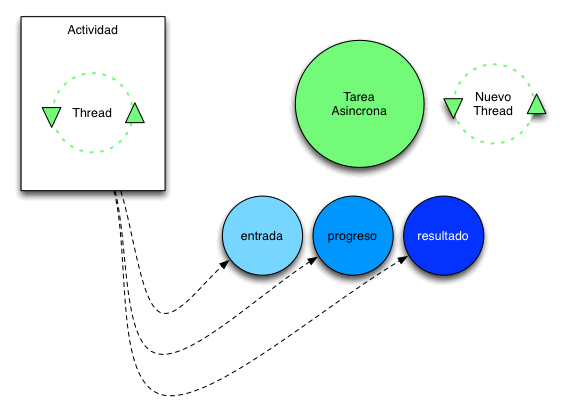
\includegraphics{figs/TareasAsincronas.png}} 
    \caption{Tareas asíncronas Android funcionamiento arquitecturajava.com} 
    \label{fig:TareasAsincronas} 
  \end{center} 
\end{figure}

En el apartado de notificaciones se le ha dado importancia a la parte del progres dialog, esto es porque mientras se está ejecutando la tarea asíncrona la actividad sigue funcionando en un thread principal. Por este motivo si se necesita esperar a que la tarea finalice y devuelva el dato a la actividad habría que usar ese progres dialog para que no se permita modificar nada hasta que acabe.
Al extender de la clase AsynTask de Android, obligará a que se tenga que implementar la función de doInbackground, esta función es la que realizará la tarea principalmente.

Aparte de esta función hay distintas funciones que serán de utilidad para trabajar con la tarea.
Una de las funciones es onPreExecute, si se implementa es la función que se realizará antes de entrar al nuevo thread, desde esta función todavía se puede modificar la parte visual de la actividad donde se ha lanzado la asynctask. Una vez se pasa al doinbackground ya no se podrá modificar.
En la función anterior es donde se suele generar el progresdialog.

Después si se quiere modificar los valores de la UI de la actividad estando desde el asynctask se necesita recurrir a dos funciones, publishProgress y onProgressUpdate.
Esas dos funciones serán las encargadas de ir modificando el valor y pasando los datos que quieren que se muestre en cada momento en la ventana de progreso que se ha lanzado en la función onPreExecute, también pueden usarse para modificar cosas que tengan que ver con la UI principal.
Y para terminar una de las funciones que más se usa es la de onPostExecute, esta función es la que se lanzará cuando se ha terminado  la función doInBackground, si se ha añadido el progres dialog hay que quitar el objeto en este punto ya que sino no se podrá tocar de nuevo la pantalla de la actividad principal.
A continuación se muestra el ciclo de vida de una asynctask

\begin{figure}[H] 
  \begin{center} 
    \scalebox{0.8}{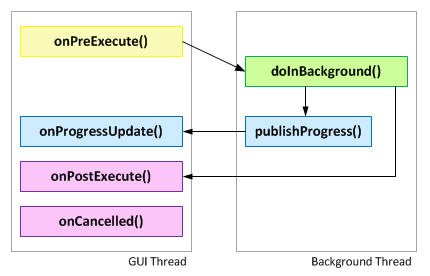
\includegraphics{figs/CicloVidaAsynctask.png}} 
    \caption{Ciclo de vida de Asynctask} 
    \label{fig:CicloVidaAsynctask} 
  \end{center} 
\end{figure}

\subsection{Backup}
\label{subsecc:Backup}

Aunque ya se ha hablado de este tema en el apartado de Google, el tema del backup en Android es un asunto muy importante, la mayoría de aplicaciones tienen algún método para guardar la información que genera el usuario.
Algunas aplicaciones hacen uso del API comentada anteriormente para realizar el backup que ofrece Google, la ventaja de esta propuesta es que la información estará guardada y se podrá recuperar la siguiente vez que el usuario quiera instalar la aplicación.

Otras aplicaciones realizan los backups directamente sobre el dispositivo, usando la tarjeta SD para guardar la información y de esta forma en el caso que el dispositivo se averíe hay una base de datos consistente que se podrá importar.
Al realizar la aplicación, en los primeros casos de uso no se le dio importancia a los backups pero después de circunstancias como fue en mí caso que se me estropeó el móvil, se echa en falta. La buena noticia fue que al tener vinculado con Google Calendar todos los exámenes se podía saber la fecha que tenían al mirar por la web.

Para que una aplicación sea útil tiene que permitir al usuario llevarse la información entre dispositivos y si por alguna circunstancia se desinstala la aplicación, que pueda instalarla de nuevo con la información que tenía anteriormente.
Hay aplicaciones que usan cuentas de usuario para volver a rellenar la base de datos en local del móvil, pidiéndole al servidor al momento de instalarlo y así no tener que estar haciendo consultas en cada momento.
Lo que se vio una buena oportunidad era juntar el uso de un API de Google junto con el backup de la aplicación. Por eso se decidió usar Google Drive.

\subsection{Debugging}
\label{subsecc:Debugging}

Cuando se está desarrollando cualquier proyecto la mejor manera de ver si funcionan las cosas es probándolas, en el caso de Android es una de las mejores opciones para que todo funcione como se espera.
Los dispositivos móviles tienen muchas variables que pueden afectar a la aplicación, las versiones o la pantalla son las más generales. Pero no son las únicas, el acceso a Internet para una aplicación que tiene que estar sincronizada a los calendarios del usuario es un factor determinante para que vaya bien.

La posición en la que se use el dispositivo suele ser un tema complicado de llevar, por eso el apartado de debugging es de los temas más importantes que hay que realizar a la hora de querer publicar una aplicación en el Google Play.
Las aplicaciones que se cuelgan al Google Play no suelen pasar por muchos controles de calidad, así que el desarrollador es el que tiene que ser el control de calidad de su aplicación. Si el propio desarrollador no está satisfecho con su trabajo es que todavía la aplicación no está disponible para salir al mercado.
Si se combina la depuración del programa junto usuarios que puedan probarla y devolver feedback, la aplicación saldrá mucho mejor de lo esperado y mucho antes que si el propio desarrollador tiene que estar haciendo todas las pruebas.

Hay aspectos que hay que probar cuando se hace el debugging si se está trabajando con un móvil. Lo mejor es ir realizando código pequeño y probarlo poco a poco en la aplicación en vez de lanzarse a programar toda la aplicación de golpe y probarlo después, en Android los errores pueden salir por muchos sitios, desde una línea no escrita en el manifest o un botón no declarado a un fallo de asignación en el TextView que se piensa que se está insertando un String y al final era un integer.

Por todos estos fallos pequeños de programación si se realiza una aplicación con varios casos de uso el error puede surgir en cualquier función por ese motivo es más sencillo realizarlo de la forma siguiente, lo primero realizar la distribución de la vista que tendrá el usuario y probar que se vea adecuadamente.

Una vez que se puede ver correctamente en todas las posiciones ya se puede pasar a darle utilidad a los botones por ejemplo. Probar con una notificación estilo Toast que funcionan correctamente los botones y que si se ha programado que salte a otra actividad lo hace sin problemas. También comprobar que pasa al darle hacia atrás y si es lógico que haga eso, ya que las actividades en Android tienen su ciclo de vida e igual no interesa que sigan vivas una vez se ha realizado alguna acción.
Cuando ya las acciones simples funcionan lo siguiente es probar si la función que se ha implementado funciona correctamente para ello en el caso que esa función devuelve  un valor, lo más rápido es añadir al Toast anterior el valor de la función, y añadir un breakpoint en la función a la hora de ejecutar las pruebas conectado al ordenador.
Con ese breakpoint cuando se lance la aplicación en la máquina virtual o el dispositivo físico podrás ejecutar el botón y se parará cuando entre en la función marcada. Se puede ir línea por línea e ir viendo que valores están cogiendo las variables.
Lo mejor en mi opinión para hacer pruebas y no estropear la batería ni el enchufe del móvil es usar una máquina virtual de Android. El problema es el consumo de memoria que tiene el uso de esta opción. Android Studio ofrece su propio administrador de máquinas virtuales de Android. Pero recomiendo usar un software que se llama Genymotion que también está adaptado a Android Studio, la ventaja de este software es que no consume tantos recursos y el móvil va más fluido.

En el caso de que se trabaje con servicios de Google las máquinas virtuales no traen por defecto los servicios de Google instalado así que hay que instalarlo en la maquina como si fuera software de terceros. Hay tutoriales por Internet e incluso webs que se dedican a subir las apks de Google play para que se puedan instalar dependiendo la versión del móvil.
El funcionamiento es sencillo solo hay que instalar 2 ficheros uno es el ARM Translation installer y el otro son los servicios de Google donde se encuentran Gmail,Google maps, youtube, etc…
Cuando se realizan estos pasos ya se tendrá un móvil Android virtual como el que se tiene físico.
Al trabajar con una máquina virtual las capturas de pantalla y grabaciones son sencillas de hacer. Y el acceso a las carpetas donde se guardan las bases de datos de la aplicación se dispone de permisos de super usuarios para entrar y descargar esos datos, cosa que si se prueba en un dispositivo físico se necesitaría rootear el teléfono para hacer lo mismo.

Una vez que los casos de uso funcionen como se tenía pensado es hora de subir la aplicación en versión alpha y hacer que los usuarios la prueben.
Para ello algo útil es hacerles un guión a la hora de realizar tareas, ver si lo pueden realizar y si les da algún tipo de fallo.
Aparte del guión es útil que ellos vayan usándola como lo usarían de normal para ver los posibles errores que puedan salir si se lanza al mercado en este momento.
Mediante software que recoge la información de la aplicación como puede ser Google Analytics o Splunk Mint se va revisando los fallos que puede estar dando la aplicación.

Durante las pruebas de Baldugenda se usó Splunk Mint, un software que todavía está en desarrollo, pero que funciona muy bien para lo que se necesitaba de la aplicación era captar los errores y decir donde fallaba sin necesitar que el usuario dijera como le había fallado.
Para la instalación dentro del terminal es muy sencilla lo único que hay que hacer es registrarse en Splunk Mint y una vez registrado crear un proyecto, agregar la librería mediante gradle o metiéndola en el proyecto.
Y después seguir los pasos que marcan en la web para hacer las llamadas a sus servicios.
Ofrece un seguimiento muy bueno dentro de la aplicación, se puede programar para que cuando un usuario pulse un botón esa acción quede recogida en su página web y después lo mostrará cuando entremos, también realiza notificaciones al email que le digamos.

El manejo es muy sencillo, se separa en 3 pestañas, la primera es donde está la información de las conexiones y de los dispositivos que tienen instalada la aplicación, la segunda pestaña es para los errores que se dan y te permite filtrarlos por fecha y te muestra un gráfico de tiempo la cantidad de errores que se han producido y la versión que en la que se ha producido el error. Y la tercera pestaña es para las configuraciones del proyecto, Splunk mint permite vincular con el proyecto que se suba a Github y hacer comentarios dentro del código, en el caso que se resuelva algún error se le puede decir a Splunk Mint que escriba en Github que se ha resuelto y en que versión ya no se produce.

\begin{figure}[H] 
  \begin{center} 
    \scalebox{0.8}{
\includegraphics{figs/SplunkMintMenu.png}} 
    \caption{Splunk Mint Menú} 
    \label{fig:SplunkMintMenu} 
  \end{center} 
\end{figure}

Los errores aparecen de la siguiente manera y es posible entrar a ellos y ver línea a línea por donde ha pasado el programa hasta llegar al error.

\begin{figure}[H] 
  \begin{center} 
    \scalebox{0.8}{
\includegraphics{figs/ErrorSplunkMint.png}} 
    \caption{Error en Splunk Mint} 
    \label{fig:ErrorSplunkMint} 
  \end{center} 
\end{figure}

También se puede configurar para que envié los errores al email que queramos.

\begin{figure}[H] 
  \begin{center} 
    \scalebox{0.8}{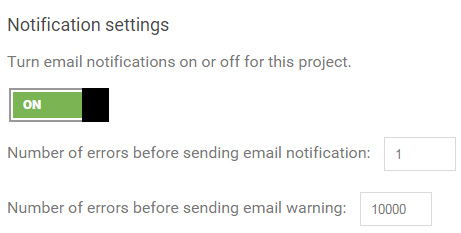
\includegraphics{figs/ConfiguracionSplunkMint.png}} 
    \caption{Configuración  Splunk Mint} 
    \label{fig:ConfiguracionSplunkMint} 
  \end{center} 
\end{figure}

Y se trabaja muy bien en el caso que sea un grupo de personas da la posibilidad de permitir ver los errores a un equipo de proyecto y enviar las notificaciones.

\subsection{Control de versiones}
\label{subsecc:Control de versiones}

Al desarrollar en Android una parte importante es mantener siempre accesible el código y saber qué cambios se han realizado, un programa, da igual el lenguaje que se esté usando y el dispositivo al que vaya enfocado es igual que un libro, no se redacta o en el caso de aplicaciones se implementa de un día para otro. Por este motivo es útil siempre usar el control de versiones para tener constancia de los cambios efectuados y si en algún momento se necesita volver a una versión anterior es más fácil realizarlo que empezar a escribir todo de nuevo, pudiendo ocasionar perdida de código por el camino y el fallo del programa.

En el caso de Android, su IDE, Android Studio facilita enormemente el trabajo con el control de versiones ya que trae incorporado opciones que permiten subir directamente el código a Github. El único requisito que pide es tener una cuenta de Github y ya estaría funcionando la subida de código con su respectivo control de versiones.
Los puntos positivos de usar el control de versiones de Github es que aparte de saber el propio desarrollador lo que ha ido generando día tras día, es un buen método para que las demás personas conozcan tus trabajos y vean si eres una persona periódica en las tareas de programación.

El propio Google usa Github para tener sus proyectos de ejemplo de los APIs que distribuye. Así que habituarse a usar esta herramienta es un buen comienzo para ver cómo trabajan los demás desarrolladores.
Aparte Github tiene plugin para múltiples programas como puede ser los de procesador de latex, una manera útil de realizar la memoria y subirla al repositorio y tenerla segura.
En el caso de usar Word 2013, ofrece también la posibilidad de marcar el control de cambios realizados, no es tan útil como Github que aparte de guardarte los cambios puedes viajar por las versiones del fichero subido pero, por lo menos se tendrá constancia de los cambios realizados ese día.

Igual que Github hay otros repositorios interesantes como puede ser gitlab, gitorious o bitbucket
Cada uno tiene sus ventajas con respecto a los otros, Github por ejemplo tiene solo repositorios públicos si se quiere usar de forma gratuita, en el caso que se quiera repositorios privados hay que pagar.
En bitbucket y los rivales de Github aprovechan eso de los repositorios privados y ofrecen uno o dos repositorios privados de forma gratuita al crear la cuenta.
De esta forma los desarrolladores pueden estar desarrollando código sin la sensación que la competencia se lo pueda quitar.
Cuando se está implementando código una buena forma de hacerlo es ir subiendo el código que funcione únicamente, por mucho que se estén haciendo pruebas, el repositorio no tiene que ser un lugar donde se guarda el código que igual un día se use.
La forma de ver el repositorio tiene que ser un lugar donde guardar el código que ya se ha probado y funciona y poco a poco ir aumentándolo hasta tener un programa consistente que aunque de fallos en ciertos momentos por lo menos son fallos de las últimas modificaciones realizadas.
También se puede ver como una manera de acceder al código sin tener que llevarlo siempre en el USB, puedes estar trabajando en el ordenador de la facultad y cuando se acaba subirlo al repositorio, al llegar a casa descargarlo y seguir trabajando.

En la situación de Baldugenda no era preciso usar Github como método de trabajo en equipo ya que el equipo estaba formado por una sola persona, pero aun y todo era una buena forma de llevar al día el tiempo que había llevado hacer cada implementación y que se había ido haciendo en cada ciclo del proyecto.
Si una aplicación la van a realizar más personas es casi imprescindible el uso de herramientas como Github, ya que no se puede estar exportando el proyecto y compartiéndolo por correo con cada modificación que se haga, porque se produciría una confusión enorme.

Un problema de usar Github es que todos los miembros del equipo tienen que saber usarlo, sino puede llevar a problemas de código corrupto al subirse o fallos que no permitirían subir el código. Pero una vez aprendido a usar Github el uso que se le puede dar es enorme, ahora permite crear páginas web explicando el proyecto que está subido y permitiendo que otros se lo descarguen o que hagan copias del proyecto en sus repositorios.
El funcionamiento de Github es por la consola si no se va a usar el plugin de Eclipse o Android Studio, aunque, se ha desarrollado aplicaciones propias para Mac  y para Windows, que hacen más fácil e interactivo la subida y descarga de los proyectos.

\subsection{Problemas al desarrollar en Android}
\label{subsecc:Problemas al desarrollar en Android}

Ya se ha hablado de los puntos importantes al crear un proyecto en Android y cosas que hay que tener en cuenta.
Al desarrollar en Android hay ciertos momentos que fallan cosas y no se encuentra solución, en este apartado se hablará de los casos que han sucedido en Baldugenda y como se han solucionado.
Uno de los casos más comunes es cuando se importa un proyecto de Github o eclipse. La mayoría de veces el IDE no detecta bien las librerías asociadas al proyecto y marca errores tanto de vistas como de la clase R de Android.
Algunas maneras de solucionarlo es instalando las APIs que requiere el proyecto, al no tenerlas descargadas e instaladas en el ordenador donde se está implementando, esto ha podido hacer que falle la compilacion y ha hecho que se falle Android Studio.
Otra solución desesperada es dentro del menú build de Android Studio la opción clean, con esto se limpiara la compilación anterior y realizará una nueva.

Un problema muy común para los que desarrollan en Eclipse son las modificaciones en el manifest o xml de vistas, hay muchas veces que se genera una actividad nueva y se olvida que para usarla tiene que estar en el manifest apuntada.
Con Android Studio este problema no pasa en gran medida ya que da la opción de generar todo de golpe, genera los layouts, modifica el manifest y genera los menús si se quiere solo dándole a un botón.
Si se es nuevo con Android como era yo al empezar la aplicación, no se conoce tan a fondo los entresijos  que depara Android a la hora de programar, uno de ellos es el uso de los servicios web.

Acostumbrado a realizar las llamadas de los servicios web donde quisiera, un error fue meterlo directamente en el hilo principal de la aplicación, al ejecutar la aplicación se bloqueaba y el debugging llevaba a unas clases creadas por Android.
Buscando por Internet explicaban que en Android toda acción que haga que la pantalla se bloquee durante un tiempo no estaba permitida hacerla en el hilo principal de la actividad.
Ese descubrimiento fue muy útil, ya que con eso aprendí  muchas cosas sobre los hilos en Android y las tareas asíncronas.

Antes se ha hablado del uso de máquinas virtuales, uno de los problemas que tiene usar máquinas virtuales son los recursos del ordenador físico que las está moviendo. En más de una ocasión se ha quedado el ordenador sin memoria por tener el Android Studio y la máquina virtual abierta, el único consejo que hay al respecto es intentar no usar máquinas virtuales muy pesadas, cuanto más alta es la API y mayores recursos se le asignan a la máquina más pesada es y más va a exigir.
Android Studio es un IDE potente para desarrollar aplicación Android el problema de esto es que al ser potente también exige mucho. Si se quiere desarrollar en Android se necesita un equipo que tenga suficiente memoria para no quedarse esperando porque se ha quedado parado al compilar el Gradle.




% Mediante los siguientes comandos, podrás compilar el conjunto de ficheros desde este mismo documento


%%% Local Variables: 
%%% mode: latex
%%% TeX-master: "../Principal"
%%% End: 


















% line in order to check if utf-8 is properly configured: áéíóúñ
\chapter{Gestión del proyecto}
\label{ch:Gestion del proyecto}
En el proyecto de Baldugenda se ha utilizado el enfoque de Lean Startup \cite{LeanStartup} para desarrollar la aplicación. Primero se ha desarrollado un \acrshort{mvp}, esto significa que se desarrolló una versión con las funcionalidades básicas en un corto periodo de tiempo. Después se empezó a añadir a los Baldusers y a pedirles el feedback, y una vez conseguido el feedback se amplió el alcance en base a la información obtenida.

Tanto la calidad del producto final como las ampliaciones realizadas se produjeron mediante las interacciones con los Baldusers. Con cada nuevo feedback recibido se realizaban cambios en Baldugenda y se les pedía opinión.

El aspecto de los Baldusers se ha tratado como un aspecto importante dentro del proyecto para el desarrollo de Baldugenda, y su calidad dentro del mercado de las aplicaciones móviles. De esta forma se ha tratado en un tema propio dentro de la memoria más detalladamente en el capítulo \ref{ch:Usuarios}.

A continuación, se hablará de la gestión del alcance dentro del proyecto, más adelante sobre la dedicación realizada en cada ciclo, después se pasará a la gestión del tiempo empleado, y para terminar el capítulo habrá un apartado de conclusiones acerca de la gestión realizada.
\newpage
\section{Gestión del alcance}
\label{secc:Gestión del alcance}

Ya se ha hablado en capítulos anteriores sobre el alcance y cómo ha ido variando dependiendo del ciclo en el que se estuviera. Este aumento del alcance ha sido gracias a los Baldusers que han ido aportando funcionalidades nuevas.
A continuación se enumerará el alcance del primer ciclo:
\begin{itemize}
	\item Creación de asignaturas indicando nombre, posibilidad de añadir enlaces y seleccionando el sistema de evaluación que se seguirá en esa asignatura. 
	\item Creación de exámenes indicando nombre, asignatura, calendario de Google Calendar, fecha y hora.
	\item Manejo básicos de calendarios de la cuenta de Google Calendar del usuario. 
	\item Los usuarios podrán escoger si quieren que se active la notificación en el examen creado dentro de Google Calendar.
	\item Borrado de exámenes desde el examen escogido.
	\item Visualizador de asignatura.
	\item Visualizador de examen.
	\item Lista de asignaturas y buscador dentro de la lista.
	\item Lista de exámenes, agrupados en asignaturas.
	\item Actividad para contactar con el desarrollador mediante email o teléfono.
	\item Uso del API de Google Calendar.
	\item Errores encontrados durante el desarrollo del prototipo resueltos.
\end{itemize}
\newpage
Una vez concluido el primer ciclo se realizó la invitación a los Baldusers y realizaron el feedback. Con el feedback devuelto se aumentó el alcance con las siguientes características:
\begin{itemize}
	\item Modificación del sistema de evaluación, enlaces y nota de una asignatura.
	\item Modificación de fecha,hora,asignatura,calendario y nota de un examen.
	\item Borrado de asignaturas que no tengan exámenes.
	\item Nuevo campo de nota en examen.
	\item Nuevo campo de nota en asignatura.
	\item Cambio de diseño de menú principal.
	\item Errores encontrados por los Baldusers resueltos.
\end{itemize}
Después del segundo ciclo, y después de añadir más Baldusers y recibir el feedback se aumentó de nuevo el alcance:
\begin{itemize}
	\item Nuevo campo de descripción en examen.
	\item Editar examen dentro de la actividad examen y desde la lista de exámenes.
	\item Editar asignatura dentro de la actividad asignatura y desde la lista de asignaturas.
	\item Borrar examen dentro de la actividad examen.
	\item Borrar asignatura dentro de la actividad asignatura y desde la lista de asignaturas.
	\item Exportar Base de datos de Baldugenda a la cuenta de Google Drive del usuario.
	\item Importar Base de datos de Baldugenda desde la cuenta de Google Drive del usuario.
	\item Uso del API de Google Drive.
	\item Errores encontrados por los Baldusers resueltos.
\end{itemize}


\newpage
\section{Gestión de costes}
\label{secc:Gestión de costes}

A continuación se detallaran mediante horas el coste humano que el proyecto ha supuesto.
Se dividirá en gestión del proyecto, aplicación Android, gestión del feedback y memoria.
Se mostrará toda la información de las horas mediante la siguiente tabla:


\begin{table}[h]
\centering
\begin{tabular}{@{}llc@{}}
\toprule
{\bf Categoria} & {\bf Tarea} & \multicolumn{1}{l}{{\bf Dedicación (h)}} \\ \midrule
Gestión del proyecto & \begin{tabular}[c]{@{}l@{}}Reuniones de control\\ Gestión de alcance\\ Adquisición de tecnologías y servicios\end{tabular} & \begin{tabular}[c]{@{}c@{}}9\\ 20\\ 6\end{tabular} \\ \midrule
Aplicación Android & \begin{tabular}[c]{@{}l@{}}Diseño gráfico de interfaz\\ Lógica de la interfaz\\ Aprendizaje API Google Calendar\\ Aprendizaje API Google Drive\\ Google Play\\ Corrección de errores\\ Pruebas\end{tabular} & \begin{tabular}[c]{@{}c@{}}20\\ 90\\ 50\\ 10\\ 4\\ 20\\ 30\end{tabular} \\ \midrule
Gestión de feedback & \begin{tabular}[c]{@{}l@{}}Motivación y promoción\\ Preparación de cuestionarios\\ Entrevistas y síntesis de los comentarios\end{tabular} & \begin{tabular}[c]{@{}c@{}}10\\ 7\\ 12\end{tabular} \\ \midrule
Memoria & \begin{tabular}[c]{@{}l@{}}Redacción\\ Aprendizaje de Latex\end{tabular} & \begin{tabular}[c]{@{}c@{}}55\\ 3\end{tabular} \\ \midrule
 & \multicolumn{1}{r}{{\bf TOTAL}} & {\bf 346}
\end{tabular}
\caption{Tabla de dedicación horaria}
\end{table}
\newpage
\section{Gestión del tiempo}
\label{secc:Gestión del tiempo}

A continuación se detallaran los hitos más importantes dentro del proyecto:

\begin{itemize}
	\item \textbf{22 de enero} Comienzo del primer ciclo
	\item \textbf{24 de enero} Alta de Baldugenda en Play Store
	\item \textbf{23 de febrero} Publicación primer prototipo funcional
	\item \textbf{5 de marzo} Baldugenda integrado con Google Calendar y subida al Play Store
	\item \textbf{26 de marzo al 7 de abril} Invitación a los Baldusers, entrevistas y feedback
	\item \textbf{27 de marzo} Finalización del primer ciclo y comienzo del segundo ciclo
	\item \textbf{23 de abril} Lanzamiento Baldugenda con primeras mejoras de Baldusers al Play Store
	\item \textbf{24 de abril al 8 de mayo} Invitación a los Baldusers tercer ciclo, entrevistas y feedback
	\item \textbf{24 de abril} Finalización del segundo ciclo y comienzo del tercer ciclo
	\item \textbf{21 de mayo} Lanzamiento Baldugenda con segundas mejoras de Baldusers al Play Store, fin de las tareas de implementación y finalización del tercer ciclo.
	\item \textbf{5 de junio} Finalización de la primera versión completa de la memoria del proyecto
\end{itemize}
\newpage
\section{Conclusiones sobre la gestión}
\label{secc:Conclusiones sobre la gestión}

Para finalizar el capítulo sobre la gestión del proyecto realizaremos un breve repaso de los apartados anteriores. Dentro de la gestión del alcance se puede observar que durante la primera fase se tuvo un mayor peso en las tareas de implementación y aprendizaje sobre las APIs de Google, por este motivo es la fase que más tiempo ha llevado dentro del proyecto. En las fases posteriores el tiempo invertido se dividió en la interacción con los Baldusers y las modificaciones que iban pidiendo que se realizaran en la aplicación.

En el apartado de costes se han dividido las categorías de la aplicación de la de los usuarios. Aunque están muy relacionadas, se invirtió un tiempo importante del proyecto en la realización de las pruebas tanto individuales como con usuarios, por este motivo esa tarea es la única en la que también están incluidas las pruebas con usuarios.
Aunque al principio se decidió trabajar con otro procesador de textos, al final acabamos decidiendo trabajar con Latex, ya que todos los aspectos de diseño y estructura serían más sencillos de realizar mediante la plantilla y se llevaría menos tiempo realizarlo.
Un aspecto muy importante para haber llevado correctamente el tiempo de cada una de las tareas, ha sido las anotaciones periódicas de cada una mediante los resúmenes de las reuniones y las subidas al Github, donde se subía una versión estable del proyecto cada 5 horas aproximadamente de trabajo.

El trabajo en fases fue muy útil de la forma en la que está pensado el desarrollo del proyecto. Al trabajar con usuarios, las fases se alargaban más que si se hubiera realizado sin el feedback de estos, aunque el tiempo que se tuvo que esperar a las respuestas de los usuarios se invirtió en probar más a fondo la aplicación, solucionar errores y poder realizar las entrevistas de una forma mas amena y calmada.
El tener separado la planificación de cada fase ha resultado muy útil a la hora de realizar una planificación general del proyecto, teniendo los hitos más importantes marcados, no ha habido ningún problema a la hora de hacer un cronograma.




































% line in order to check if utf-8 is properly configured: áéíóúñ
\chapter{Ondorioak/conclusiones}































% line in order to check if utf-8 is properly configured: áéíóúñ

\chapter{Propuestas de extension y mejoras futuras}

Algo que no hay que olvidar de una aplicación es que su ciclo de vida no termina cuando se finaliza un proyecto. Todas las aplicaciones para dispositivos móviles necesitan de un mantenimiento, dentro de este mantenimiento están incluidas las nuevas versiones de la aplicación añadiendo funcionalidades nuevas o arreglando las ya existentes.
En este capítulo se detallarán las propuestas que se han planteado añadir en Baldugenda.
Se separará en dos apartados: por un lado las propuestas de extensión donde se hablará sobre cambios importantes dentro de Baldugenda, y por otro lado se hablará sobre las mejoras que se podrían realizar en la aplicación.
\newpage
\section{Propuestas de extensión}

Las propuestas citadas a continuación son ideas aportadas por los Baldusers e ideas de origen propio, para que sirvan como propuesta para dar continuidad al trabajo presentado en esta memoria. 
\begin{itemize}
	\item Ya que Baldugenda esta dirigido a los estudiantes universitarios, añadir dentro de los destinatarios de la aplicación a los profesores para que puedan llevar al día los exámenes y compartirlos con los estudiantes.
	\item Durante la fase de pruebas se comprobó que el funcionamiento de Baldugenda funcionaria correctamente en los institutos realizando modificaciones como puede ser agregar trabajos y deberes.
	\item La ampliación de las funcionalidades de Baldugenda haciéndolas accesibles a las personas con discapacidad seria una buena forma de conseguir usuarios que la mayoría de aplicaciones dejan de lado.
	\item La realización de Widgets para el móvil de la aplicación, donde se podría visualizar los exámenes y las asignaturas sin necesidad de abrir la aplicación y de esta manera poder realizar notificaciones al usuario sin la necesidad de usar las de Google Calendar.
	\item La implementación de Baldugenda en distintos dispositivos Android, como SmartTv o Smartwatch.
	\item Migración de Baldugenda a otros sistemas operativos, siendo el prioritario IOs.
	\item Implementación de version web de Baldugenda.
	\item Sincronización de Baldugenda con Gaur para acceder a las asignaturas.
\end{itemize}
\newpage
\section{Propuestas de mejora}

Las propuestas de mejora son ideas que mejorarían el producto actual, Baldugenda.
A continuación se exponen las ideas aportadas por los Baldusers junto con ideas propias que mejorarían Baldugenda si se le diera continuidad al trabajo. 
\begin{itemize}
	\item La implementación de una actividad para visualizar los eventos en forma de calendario.
	\item Nuevos campos dentro de una asignatura como podrían ser trabajos, tutorías, exposiciones.
	\item Añadir horario dentro de una asignatura.
	\item Modificar el diseño de la aplicación y de sus actividades para que cada sección tuviera un color propio para distinguir en que parte se esta en cada momento.
	\item Realizar la aplicacion en distintos idiomas, esta propuesta se tuvo en cuenta pero no se pudo realizar por falta de tiempo. Se dejó todo preparado para la traducción de las palabras por medio de los ficheros String.xml
	\item Añadir el material design a la aplicación.
	\item Añadir mas opciones a la hora de crear un examen en Google Calendar, como puede ser invitar a gente a ese evento o configurar una notificación a una dirección de correo.
	\item Compartir calendarios y poder descargar calendarios ya existentes.
\end{itemize}
\chapter{hola}
\section{fallo}


\noappendicestocpagenum
\appendixpage
\addappheadtotoc
\appendix
% Adjustments headers
\pagestyle{fancy}
\fancyhead[LO]{\leftmark}
\ifdefined\euskaraz
	\fancyhead[RE]{\emph{\thechapter eranskina}}
\else
	\fancyhead[RE]{\emph{Anexo \thechapter}}
\fi
\renewcommand{\headrulewidth}{0.5pt}

% \chapter{Eranskinaren izenburua/título del anexo}




































% line in order to check if utf-8 is properly configured: áéíóúñ



\backmatter

\bibliography{gap-pfg}

% In case we are using a glossary
% \glstoctrue
% \glsaddall
% \printglossaries

\end{document}
% line in order to check if utf-8 is properly configured: áéíóúñ
